\documentclass[lang=cn,newtx,10pt,scheme=chinese]{elegantbook}

\title{数学分析学习笔记}
\subtitle{复习整理笔记}

\author{阮炜挺}
\institute{宁波大学数学与统计学院}
\date{}

\extrainfo{Given yourself an epsilon of room!}

\setcounter{tocdepth}{3}

\cover{cover.jpg}

% 本文档命令
\usepackage{array}
\newcommand{\ccr}[1]{\makecell{{\color{#1}\rule{1cm}{1cm}}}}

% 修改标题页的橙色带
\definecolor{customcolor}{RGB}{32,178,170}
\colorlet{coverlinecolor}{customcolor} 
\usepackage{cprotect}
\usepackage{tikz}
\usetikzlibrary{calc}
\addbibresource[location=local]{reference.bib} % 参考文献,不要删除

\begin{document}

\maketitle
\frontmatter

\tableofcontents

\mainmatter

\chapter{公式大全}
\section{常见函数的泰勒展开式}		

\subsection*{几何级数}
\begin{align*}
    \displaystyle \frac{1}{1 - x} &= 1 + x + x^2 + x^3 + \cdots + x^n + o(x^n) \\
    \displaystyle \frac{1}{1 + x} &= 1 - x + x^2 - x^3 + \cdots + (-1)^n x^n + o(x^n)
\end{align*}

\subsection*{指数和对数函数}
\begin{align*}
    \displaystyle & e^x = 1 + x + \frac{x^2}{2!} + \frac{x^3}{3!} + \cdots + \frac{x^n}{n!} + o(x^n) \\
    \displaystyle & \ln(1 + x) = x - \frac{x^2}{2} + \frac{x^3}{3} - \frac{x^4}{4} + \cdots + (-1)^{n+1} \frac{x^n}{n} + o(x^n)
\end{align*}

\subsection*{幂函数}
\begin{align*}
    \displaystyle (1 + x)^a &= 1 + a x + \frac{a(a-1)}{2!} x^2 + \cdots + \binom{a}{n} x^n + o(x^n) \\
    \displaystyle \sqrt{1 + x} &= \boxed{1 + \frac{1}{2}x - \frac{1}{8}x^2} + \frac{1}{16}x^3 + \cdots + \frac{(-1)^{n+1} (2n-3)!!}{2^n n!} x^n + o(x^n)
\end{align*}

\subsection*{三角函数}
\begin{align*}
    \displaystyle \sin x &= x - \frac{x^3}{3!} + \frac{x^5}{5!} - \cdots + (-1)^n \frac{x^{2n+1}}{(2n+1)!} + o(x^{2n+2}) \\
    \displaystyle \cos x &= 1 - \frac{x^2}{2!} + \frac{x^4}{4!} - \cdots + (-1)^n \frac{x^{2n}}{(2n)!} + o(x^{2n+1}) \\
    \displaystyle \tan x &= \boxed{x + \frac{x^3}{3} + \frac{2}{15}x^5} + \cdots + \frac{B_{2n} (-4)^n (1 - 4^n)}{(2n)!} x^{2n - 1} + o(x^{2n})
\end{align*}

\subsection*{反三角函数}
\begin{align*}
    \displaystyle \arcsin x &= \boxed{x + \frac{x^3}{6}} + \frac{3}{40}x^5 + \cdots + \frac{(2n)!}{4^n (n!)^2 (2n + 1)} x^{2n+1} + o(x^{2n+2}) \\
    \displaystyle \arctan x &= x - \frac{x^3}{3} + \frac{x^5}{5} - \cdots + (-1)^n \frac{x^{2n+1}}{2n+1} + o(x^{2n+2})
\end{align*}

\newpage
\section{常见三角恒等式}

\subsection*{积化和差公式}
\begin{align*}
    \sin A \sin B &= \frac{1}{2}[\cos(A - B) - \cos(A + B)] \\
    \cos A \cos B &= \frac{1}{2}[\cos(A - B) + \cos(A + B)] \\
    \sin A \cos B &= \frac{1}{2}[\sin(A + B) + \sin(A - B)] \\
    \cos A \sin B &= \frac{1}{2}[\sin(A + B) - \sin(A - B)]
\end{align*}

\subsection*{和差化积公式}
\begin{align*}
    \sin A + \sin B &= 2 \sin\left( \frac{A + B}{2} \right) \cos\left( \frac{A - B}{2} \right) \\
    \sin A - \sin B &= 2 \cos\left( \frac{A + B}{2} \right) \sin\left( \frac{A - B}{2} \right) \\
    \cos A + \cos B &= 2 \cos\left( \frac{A + B}{2} \right) \cos\left( \frac{A - B}{2} \right) \\
    \cos A - \cos B &= -2 \sin\left( \frac{A + B}{2} \right) \sin\left( \frac{A - B}{2} \right)
\end{align*}

\subsection*{基本恒等式}
\[
\sin^2 x + \cos^2 x = 1
\]
\[
1 + \tan^2 x = \sec^2 x
\]
\[
1 + \cot^2 x = \csc^2 x
\]

\subsection*{倒数关系}
\[
\sec x = \frac{1}{\cos x} \quad \csc x = \frac{1}{\sin x} \quad \cot x = \frac{1}{\tan x}
\]

\subsection*{倍角公式}
\[
\sin 2x = 2 \sin x \cos x
\]
\[
\cos 2x = \cos^2 x - \sin^2 x = 2\cos^2 x - 1 = 1 - 2\sin^2 x
\]
\[
\tan 2x = \frac{2\tan x}{1 - \tan^2 x}
\]

\subsection*{半角公式}
\[
\sin^2 \frac{x}{2} = \frac{1 - \cos x}{2}
\]
\[
\cos^2 \frac{x}{2} = \frac{1 + \cos x}{2}
\]
\[
\tan \frac{x}{2} = \frac{\sin x}{1 + \cos x} = \frac{1 - \cos x}{\sin x}
\]

\subsection*{三角函数万能代换}

令 $t = \tan \frac{x}{2}$。

则
$$ \tan x = \frac{2 \tan \frac{x}{2}}{1 - \tan^2 \frac{x}{2}} = \frac{2t}{1 - t^2} $$

根据勾股定理,我们有 $(2t)^2 + (1 - t^2)^2 = 4t^2 + 1 - 2t^2 + t^4 = t^4 + 2t^2 + 1 = (1 + t^2)^2$。

根据三角函数的几何意义,绘出三边关系图:

\begin{center}
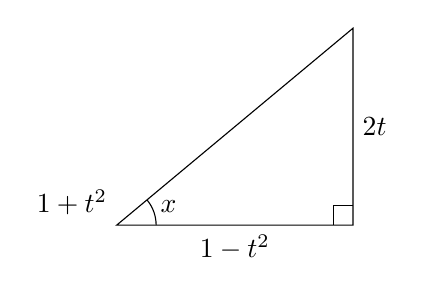
\begin{tikzpicture}
    % 定义坐标点
    \coordinate (A) at (0,0);
    \coordinate (B) at (3,0);      % 直角顶点
    \coordinate (C) at (3,2.5);

    % 绘制三角形
    \draw (A) -- (B) -- (C) -- cycle;

    % 标记直角 (在点 B 处)
    \def\rightanglesize{0.25cm} % 定义直角标记的大小 (添加了单位cm)
    % 计算直角标记的三个点:
    % B_h: 从B点沿水平向左移动 \rightanglesize
    % B_v: 从B点沿垂直向上移动 \rightanglesize
    % B_c: 直角标记的实际角点
    \coordinate (B_h) at ($(B)+(-\rightanglesize,0)$);
    \coordinate (B_v) at ($(B)+(0,\rightanglesize)$);
    \coordinate (B_c) at ($(B)+(-\rightanglesize,\rightanglesize)$);
    % 绘制直角标记符
    \draw (B_h) -- (B_c) -- (B_v);

    % 标记边长
    \node[below] at ($(A)!0.5!(B)$) {$1 - t^2$};
    \node[right] at ($(B)!0.5!(C)$) {$2t$};
    \node[above left, midway, sloped] at ($(A)!0.5!(C)$) {$1 + t^2$};

    % 标记角度x (在点 A 处)
    \pgfmathsetmacro{\oppositeSide}{(2.5)} % 对边长度 (y_C - y_A)
    \pgfmathsetmacro{\adjacentSide}{(3)}   % 邻边长度 (x_B - x_A)
    \pgfmathsetmacro{\angleValue}{atan(\oppositeSide/\adjacentSide)} % 计算角度 (单位: 度)
    \def\arcradius{0.5cm} % 定义圆弧半径
    % 绘制角度弧线
    \draw ($(A)+(\arcradius,0)$) arc (0:\angleValue:\arcradius);
    % 标记角度x的标签,位置在角平分线上,距离A点 \arcradius + 0.2cm
    \node at ($(A)+(\angleValue/2:\arcradius+0.2cm)$) {$x$};

\end{tikzpicture}
\end{center}

因此,
$$ \sin x = \frac{2t}{1 + t^2} $$
$$ \cos x = \frac{1 - t^2}{1 + t^2} $$

而 $t = \tan \frac{x}{2}$,所以 $x = 2 \arctan t$。

则
$$ dx = \frac{2}{1 + t^2} dt $$

最终结果:
\begin{align*}
&\sin x = \frac{2t}{1 + t^2} \\
&\cos x = \frac{1 - t^2}{1 + t^2} \\
&\tan x = \frac{2t}{1 - t^2} \\
&x = 2 \arctan t \\
&dx = \frac{2}{1 + t^2} dt
\end{align*}


\section{常见积分公式}

\subsection*{重要积分公式}
\[
\int \ln x \, dx = x \ln x - x + C
\]

\begin{equation*}
    \boxed{
    \int \frac{1}{\sqrt{x^2 + 1}} \, dx = \ln|x + \sqrt{x^2 + 1}| + C
    }
\end{equation*}

\begin{equation*}
    \boxed{
    \int \frac{1}{\sqrt{x^2 - 1}} \, dx = \ln|x + \sqrt{x^2 - 1}| + C
    }
\end{equation*}

\subsection*{三角函数积分}
\[
\int \sec^2 x \, dx = \tan x + C
\]
\[
\int \csc^2 x \, dx = -\cot x + C
\]
\[
\int \sec x \tan x \, dx = \sec x + C
\]
\[
\int \csc x \cot x \, dx = -\csc x + C
\]

\subsection*{反三角函数积分}
\[
\int \frac{1}{\sqrt{1 - x^2}} \, dx = \arcsin x + C
\]

\[
\int \frac{-1}{\sqrt{1 - x^2}} \, dx = \arccos x + C
\]

\[
\int \frac{1}{1 + x^2} \, dx = \arctan x + C
\]

\[
\int \frac{1}{x \sqrt{x^2 - 1}} \, dx = \mathrm{arcsec} x + C \quad (|x| > 1)
\]

\vspace{3mm}
\begin{remark}
    由于$\arcsin x + \arccos x =\frac{\pi}{2}$,那么第二个式子其实也可以写成$\int \frac{-1}{\sqrt{1 - x^2}} \, dx =  - \arcsin x + C$
\end{remark}
\vspace{5mm}
\begin{note}
    利用以上结果,我们还可以进行特殊代换,得到一些常用的积分公式:
    \[
    \int \frac{1}{a^2 + x^2} \, dx = \frac{1}{a} \arctan\frac{x}{a} + C
    \]
    \[
    \int \frac{1}{\sqrt{a^2 - x^2}} \, dx = \arcsin\frac{x}{a} + C
    \]
    \[
    \int \frac{1}{x^2 - a^2} \, dx = \frac{1}{2a} \ln\left|\frac{x - a}{x + a}\right| + C
    \]
\end{note}








\chapter{实数完备性定理}
\section{定理叙述}
\begin{theorem}[确界原理]
任何非空集 \( E \subset \mathbb{R} \),若它有上界,则必有上确界 \(\sup E \in \mathbb{R}\)。(等价地,若有下界,则必有下确界。)
\end{theorem}

\begin{theorem}[单调有界原理]
任何单调递增、有上界的序列 \(\{x_n\} \subset \mathbb{R}\),必有极限 \(\lim \limits_{n \to \infty} x_n \in \mathbb{R}\)。(等价地,单调递减有下界也必有极限。)(所谓有极限,指有有限极限,下同。)
\end{theorem}

\begin{theorem}[Cauchy收敛原理]
序列 \(\{x_n\} \subset \mathbb{R}\) 收敛的充分必要条件是
\[
\forall \varepsilon > 0, \exists N > 0, \text{当 } m, n > N \text{时,有 } |x_n - x_m| < \varepsilon.
\]
\end{theorem}

\begin{theorem}[致密性定理(Bolzano-Weierstrass定理)]\label{thm:bolzano-weierstrass}
\underline{(a) 有界数列的定义}:
设 \(\{x_n\}\) 为一数列,若 \(\exists M > 0\),满足对任意正整数 \(n\),\(|x_n| \leq M\),则称 \(\{x_n\}\) 为\emph{有界数列}。

\underline{(b) 定理内容}:
设 \(\{x_n\}\) 为一有界数列,则 \(\{x_n\}\) 一定有收敛子列。即存在 \(\{x_{n_k}\} \subset \{x_n\}\),满足 \(\lim\limits_{k \to \infty} x_{n_k}\) 存在。反之若 \(\{x_n\}\) 的任何子列都不收敛,则 \(\lim\limits_{n \to \infty} x_n = \infty\)。
\end{theorem}

\begin{theorem}[聚点定理]\label{thm:accumulation-point}
\underline{(a) 聚点的定义}:
设 \(E \subset \mathbb{R}\),\(x_0 \in \mathbb{R}\) 满足:对任意 \(\varepsilon > 0\),有
\[
\big( (x_0 - \varepsilon, x_0 + \varepsilon) \setminus \{x_0\} \big) \cap E \neq \varnothing,
\]
则称 \(x_0\) 为 \(E\) 的\emph{聚点}。记 \(E'\) 为 \(E\) 的所有聚点构成的集合。

\underline{(b) 定理内容}:
设 \(E\) 是无穷有界集合,则 \(E\) 至少有一个聚点(即 \(E' \neq \varnothing\))。
\end{theorem}

\begin{theorem}[闭区间套定理]
\underline{定义}:\\
设有无穷多个闭区间 \( [a_n, b_n],\ n = 1, 2, 3, \ldots \),满足以下两个条件:
\begin{enumerate}
    \item \( [a_{n+1}, b_{n+1}] \subseteq [a_n, b_n] \)
    \item \( \lim\limits_{n \to \infty} (b_n - a_n) = 0 \)
\end{enumerate}
将这一无穷多个闭区间所构成的集合 \(\{[a_n, b_n]\}\) 称为一个\emph{闭区间套},简称\emph{区间套}。

\underline{定理内容}:\\
若 \(\{[a_n, b_n]\}\) 是一个闭区间套,则存在唯一实数 \(\xi\) 满足:
\[
\xi \in [a_n, b_n], \quad \forall n = 1, 2, 3, \ldots
\]
且
\[
\lim_{n \to \infty} a_n = \lim_{n \to \infty} b_n = \xi.
\]
\end{theorem}

\begin{theorem}[有限覆盖定理]
\underline{(a) 定义}:
设 \( E \subset \mathbb{R} \),\(\{O_\lambda : \lambda \in \Lambda\}\) 是一族开区间,若满足
\[
\bigcup_{\lambda \in \Lambda} O_\lambda \supseteq E,
\]
则称 \(\{O_\lambda : \lambda \in \Lambda\}\) 为 \( E \) 的\emph{开覆盖}。若 \( E \) 的\emph{任何}开覆盖都存在有限子覆盖(即存在有限个 \(O_{\lambda_1},...,O_{\lambda_n}\) 仍覆盖 \(E\)),则称 \( E \) 是\emph{紧的}。

\underline{(b) 定理内容}:
任何有界闭区间 \([a, b]\) 都是紧的(闭区间上的任一开覆盖必存在有限子覆盖)。\\
\underline{(c) 等价描述}:
设 \(\{ \Delta \}\) 是一组开区间,若 \(\forall x \in [a,b]\),\(\exists \Delta_x \in \{ \Delta \}\),使得 \(x \in \Delta_x\),则称 \(\{ \Delta \}\) 为闭区间 \([a,b]\) 的一个开覆盖。定理指出,\([a,b]\) 的任一开覆盖 \(\{ \Delta \}\) 中,必存在有限子集 \(\{\Delta_1, \Delta_2, \cdots, \Delta_r\} \subset \{ \Delta \}\),\(\{\Delta_1, \Delta_2, \cdots, \Delta_r\}\) 仍为 \([a,b]\) 的一个开覆盖(称之为有限子覆盖)。
\end{theorem}

\begin{theorem}[Dedekind分割定理]
若将实数分为上、下(非空的)两组:\(A'\) 和 \(A\),使得
\begin{enumerate}
    \item 每个实数必在,且仅在两组之一;
    \item 上组 \(A'\) 中的每个数必大于下组 \(A\) 中的每个数,
\end{enumerate}
则称 \(A\) 和 \(A'\) 组成一Dedekind分割,记作 \(A|A'\)。每个 \(A|A'\) 确定唯一的实数 \(\xi\)。下面称它为分割点。

Dedekind定理指出,此时
\begin{enumerate}
    \item 要么 \(\xi \in A\),则下组 \(A\) 中有最大值 \(\xi\),而上组 \(A'\) 中无最小值;
    \item 要么 \(\xi \in A'\),则下组 \(A\) 中无最大值,而上组 \(A'\) 中有最小值 \(\xi\)。
\end{enumerate}
该定理非常直观,意即:在数轴任何地方,用法平面去截,必截得唯一的实数 \(\xi\)(表明实轴连续,无空缺)。该实数 \(\xi\) 将数轴分成 \(A|A'\) 两半,要么 \(\xi \in A\),要么 \(\xi \in A'\)。
\end{theorem}

我们先证明致密性定理\ref{thm:bolzano-weierstrass}与聚点定理\ref{thm:accumulation-point}的等价性,接下来的互证里,只涉及其中之一。

聚点定理\ref{thm:accumulation-point}$\Rightarrow$致密性定理\ref{thm:bolzano-weierstrass}
\begin{proof}
    设 $\{a_n\}$ 是 $\mathbb{R}$ 中的有界列。
    
    考虑集合 $E := \{a_n \mid n \geq 1\}$,则 $E$ 是有界集。
    
    \begin{itemize}
        \item \textbf{情形 1.} 若 $E$ 是有限集,则必有某个$a$ 在 $\{a_n\}$ 中出现无限多次。将相应的项取出,形成 $\{a_n\}$ 的一个取常值 $a$ 的子列。显然,该子列收敛到 $a$。
        
        \item \textbf{情形 2.} 若 $E$ 是无限集,则 $E$ 有聚点,设为 $\xi$。构造严格递增的正整数列 $\{n_k\}$ 如下:
        \begin{itemize}
            \item 在区间 $(\xi - 1, \xi + 1)$ 中取 $n_1 \geq 1$,使得 $a_{n_1} \in (\xi - 1, \xi + 1)$;
            \item 在区间 $(\xi - \frac{1}{2}, \xi + \frac{1}{2})$ 中取 $n_2 > n_1$,使得 $(\xi - \frac{1}{2}, \xi + \frac{1}{2})$;
            \item 依此类推,对任意 $k$,在区间
            $$ \left( \xi - \frac{1}{k}, \xi + \frac{1}{k} \right) $$
            中取 $n_k > n_{k-1}$,使得 $a_{n_k} \in \left( \xi - \frac{1}{k}, \xi + \frac{1}{k} \right)$。
        \end{itemize}
        由此可得子列 $\{a_{n_k}\}$ 满足:
        $$ \lim_{k \to \infty} a_{n_k} = \xi $$
        因此 $\{a_{n_k}\}$ 是 $\{a_n\}$ 的收敛子列。
    \end{itemize}
    $\hfill \blacksquare$
    \end{proof}

致密性定理\ref{thm:bolzano-weierstrass}$\Rightarrow$聚点定理\ref{thm:accumulation-point}:
\begin{proof}
    设点集 $S$ 为一有界无穷点集,依次任取 $S$ 中不重复的点(保证极限不为孤立点)构成数列 $\{a_n\}$,根据致密性定理,必存在收敛子列满足 
$\lim\limits_{k \to \infty} a_{n_k} = \xi,$
由极限定义,$\forall \varepsilon > 0$,$\exists N \in \mathbb{N}^+$,使 $k > N$ 时有 
$|a_{n_k} - \xi| < \varepsilon,$因而 $\xi$ 是聚点。$\hfill\blacksquare$
\end{proof}

\newpage 
对于Dedekind 分割定理,我们做如下的详细说明。
    \begin{definition}[有理数集的切割]
    设两个非空有理数集合 $A$ 和 $B$ 满足:

    \begin{itemize}
    \item $ \mathbb{Q} = A \cup B $
    \item $ \forall a \in A, \forall b \in B: a < b $
    \end{itemize}

    则称 $A, B$ 构成 $\mathbb{Q}$ 的一个切割,记为:
    \[
    A \mid B
    \]
    \end{definition}
    \begin{example}
    判断以下是否为有理数集 $\mathbb{Q}$ 的切割

    考虑以下四组区间,对每一组分别取两个区间内的有理数构成两个集合,判断是否构成 $\mathbb{Q}$ 的一个切割:
    \begin{align*}
    & (-\infty, 2] , (2, +\infty) \\
    & (-\infty, 2) , [2, +\infty) \\
    & (-\infty, \sqrt{2}) , (\sqrt{2}, +\infty) \\
    & (-\infty, 2] , [2, +\infty)
    \end{align*}

    前三组能构成 $\mathbb{Q}$ 的切割,最后一组不能构成切割。
    \end{example}
    
    \begin{remark}
        从上述例子中可以归纳 Dedekind 切割的四种可能情况:

        \begin{enumerate}
        \item $A$ 有最大数,$B$ 无最小数
        \item $A$ 无最大数,$B$ 有最小数
        \item $A$ 无最大数,$B$ 无最小数
        \item $A$ 有最大数,$B$ 有最小数(不成立)
        \end{enumerate}

        设 \( A \) 有最大数时,最大数为 \( a_0 \),\( B \) 有最小数时,最小数为 \( b_0 \)。
        这四种情况与前面提到的具体例子相对应,第四种情形不可能发生,下面来证明。
        假设第四种情况成立,则 $\frac{a_0 + b_0}{2}$是有理数且  
        $a_0 < \frac{a_0 + b_0}{2} < b_0$
        这样一个既不属于 \( A \) 也不属于 \( B \) 的有理数存在说明  
        $A \cup B \neq Q$,
        与切割的定义相矛盾。
    \end{remark}    

    情况1可以确定一个有理数$a_0$,情况2可以确定一个有理数$b_0$ ,但情况3则没有确定任何有理数,这意味着全体有理数的两个补集之间有空隙,我们将这个空隙定义为无理数.这样我们引入一种对无理数的定义方法.
    \begin{definition}[定义无理数]
    设 $A\mid B$ 是有理数集 $\mathbb{Q}$ 的一个切割,且满足:$A$ 无最大数,$B$ 无最小数.
    则 $A \mid B$ 确定了一个无理数 $c$,满足:
    $\forall a \in A, \forall b \in B: a < c < b$.
    该 $c$ 可视为填补有理数间“空隙”的无理数。
    \end{definition}
    \begin{definition}[Dedekind原理]
        设 $A, B$ 是实数域 $\mathbb{R}$ 的两个子集,它们满足以下三个条件:
        
        \begin{enumerate}
        \item[(a)] 不空:$A \neq \emptyset$ 且 $B \neq \emptyset$;
        \item[(b)] 不漏:$A \cup B = \mathbb{R}$;
        \item[(c)] 不乱:对 $\forall x \in A, y \in B$ 都成立 $x < y$;
        \end{enumerate}
        
        则称 $(A|B)$ 为实数域的一个 \textsf{Dedekind} 分割,$A$ 为分割的下集,$B$ 为分割的上集。
    \end{definition}

    \begin{theorem}[Dedekind分割定理]
        设 $(A \mid B)$ 是实数域的一个 \textsf{Dedekind} 分割,则或者下集 $A$ 中有最大数,或者上集 $B$ 中有最小数。

        等价描述:
        设 $(A \mid B)$ 是实数域的一个 \textsf{Dedekind} 分割,则存在实数 $c$ 使得
        $x \leq c \leq y \quad \forall x \in A, \forall y \in B$
        成立。实数 $c$ 称为分划 $(A\mid B)$ 的分界点,且 $c$ 是唯一的。
    \end{theorem}


\newpage
\section{确界原理}
\begin{theorem*}[确界原理]
    任何非空集 \( E \subset \mathbb{R} \),若它有上界,则必有上确界 \(\sup E \in \mathbb{R}\)。(等价地,若有下界,则必有下确界。)
\end{theorem*}

\begin{problem}
    用单调有界原理证明确界原理。
\end{problem}

\begin{proof}
    设数集 $S$ 非空有上界,即存在 $a \in S$,不妨设数 $a$ 不是 $S$ 的上界,存在数 $b$ 是 $S$ 的上界。
    
    将区间 $[a,b]$ 二等分:
    
    若中点 $\frac{a+b}{2} \in S$,则取 $a_1 = \frac{a+b}{2}, b_1 = b$;
    
    若中点 $\frac{a+b}{2} \notin S$,则取 $a_1 = a, b_1 = \frac{a+b}{2}$,得小区间 $[a_1, b_1]$。
    
    如此无限继续下去,得两个数列 $\{a_n\}, \{b_n\}$,其中 $a_n \in S$ 且单调递增有上界 $b$,$b_n$ 单调递减有下界 $a_1$,且 $\lim\limits_{n \to \infty} (b_n - a_n) = \lim\limits_{n \to \infty} \frac{b-a}{2^n} = 0$。
    
    由单调有界定理知存在 $\xi$,使得 $\lim\limits_{n \to \infty} a_n = \xi$,又由 $\lim\limits_{n \to \infty} (b_n - a_n) = 0$ 知 $\lim\limits_{n \to \infty} b_n = \xi$。
    因 $\{b_n\}$ 是 $S$ 的上界,所以 $\forall x \in S$ 有 $x \leq b_n$ ($n=1,2,\cdots$),令 $n \to \infty$ 得 $x \leq \lim\limits_{n \to \infty} b_n = \xi$,
    所以 $\xi$ 为 $S$ 的上界。
    
    因 $\forall \varepsilon > 0$,由 $\lim\limits_{n \to \infty} a_n = \xi$ 知,存在 $N$,当 $n > N$ 时有 $\xi - \varepsilon < a_n$,即 $\xi - \varepsilon < a_{N+1}$,
    又对所有的 $a_n \in S$,即存在 $S$ 中的某个数 $a_{N+1}$,使得 $\xi - \varepsilon < a_{N+1}$,故 $\xi$ 为 $S$ 的最小上界。所以 $\xi = \sup S$。
    
    同理可证非空有下界的数集,必有下确界。$\hfill\blacksquare$
\end{proof}
    
\begin{problem}
    用Cauchy收敛原理证明确界原理。
\end{problem}

\begin{proof}
    设数集 $S$ 非空有上界,即存在 $a \in S$,不妨设数 $a$ 不是 $S$ 的上界,存在数 $b$ 是 $S$ 的上界。
    
    将区间 $[a, b]$ 二等分:
    
    若中点 $\frac{a+b}{2}$ 是 $S$ 的上界,则取 $a_1 = a, b_1 = \frac{a+b}{2}$;
    
    若中点 $\frac{a+b}{2}$ 不是 $S$ 的上界,则取 $a_1 = \frac{a+b}{2}, b_1 = b$,得小区间 $[a_1, b_1]$。
    
    如此无限继续下去,得两个数列 $\{a_n\}, \{b_n\}$,其中 $a_n$ 不是 $S$ 的上界,$b_n$ 是 $S$ 的上界,且
    $
    \lim\limits_{n \to \infty} (b_n - a_n) = \lim\limits_{n \to \infty} \frac{b-a}{2^n} = 0.
    $
    
    下面证明 $\{a_n\}$ 满足柯西收敛准则。

    由 $\lim\limits_{n \to \infty} (b_n - a_n) = 0$ 知 $\forall \varepsilon > 0, \exists N, n > N$ 时有 $|b_n - a_n| < \varepsilon$;又 $a_n \leq a_{n+1} \leq b_{n+1} \leq b_n$,从而 $\forall p$ 有 $|a_{n+p} - a_n| \leq |b_n - a_n| < \varepsilon$,故 $\{a_n\}$ 满足柯西收敛准则,从而有极限。
    
    设 $\lim\limits_{n \to \infty} a_n = \xi$,从而也得到 $\lim\limits_{n \to \infty} b_n = \xi$。
    
    再证明 $\xi = \sup S$。
    
    对任意的 $n$ 和任意的 $x \in S$,因 $b_n$ 是 $S$ 的上界,所以有 $x \leq b_n$,令 $n \to \infty$ 得 $x \leq \lim\limits_{n \to \infty} b_n = \xi$,所以 $\xi$ 为 $S$ 的上界。
    而 $\forall \varepsilon > 0$,由 $\lim\limits_{n \to \infty} a_n = \xi$ 知,存在 $N$,当 $n > N$ 时有 $\xi - \varepsilon < a_n$,即 $\xi - \varepsilon < a_{N+1}$。
    
    又对所有的 $a_n \in S$,即存在 $S$ 中的某个数 $a_{N+1}$,使得 $\xi - \varepsilon < a_{N+1}$,故 $\xi$ 为 $S$ 的最小上界。所以 $\xi = \sup S$。
    
    同理可证非空有下界的数集,必有下确界。
    $\hfill\blacksquare$
\end{proof}    

\begin{problem}
    用闭区间套定理证明确界原理。
\end{problem}

\begin{proof}
    设数集 $S$ 非空有上界,即存在 $a \in S$,不妨设数 $a$ 不是 $S$ 的上界,存在数 $b$ 是 $S$ 的上界。
    
    将区间 $[a, b]$ 二等分:
    
    若中点 $\frac{a+b}{2}$ 是 $S$ 的上界,则取 $a_1 = a, b_1 = \frac{a+b}{2}$;
    
    若中点 $\frac{a+b}{2}$ 不是 $S$ 的上界,则取 $a_1 = \frac{a+b}{2}, b_1 = b$,得小区间 $[a_1, b_1]$。
    
    如此无限继续下去,得一区间套 $[a_n, b_n]$,其中 $a_n$ 不是 $S$ 的上界、$b_n$ 是 $S$ 的上界,且
     $
    \lim\limits_{n \to \infty} (b_n - a_n) = \lim\limits_{n \to \infty} \frac{b-a}{2^n} = 0.
    $
    故由区间套定理知,存在唯一的一点 $\xi$,使得 $\xi \in [a_n, b_n] (n=1,2,\cdots)$,且
     $
    \lim\limits_{n \to \infty} a_n = \lim\limits_{n \to \infty} b_n = \xi.
    $
    
    对任意的 $x \in S$,因 $b_n$ 是 $S$ 的上界,所以有 $x \leq b_n$,令 $n \to \infty$ 得 $x \leq \lim\limits_{n \to \infty} b_n = \xi$,所以 $\xi$ 为 $S$ 的上界。
    
    而 $\forall \varepsilon > 0$,由 $\lim\limits_{n \to \infty} a_n = \xi$ 知,存在 $N$,当 $n > N$ 时有 $\xi - \varepsilon < a_n$,即 $\xi - \varepsilon < a_{N+1}$,又对所有的 $a_n \in S$,即存在 $S$ 中的某个数 $a_{N+1}$,使得 $\xi - \varepsilon < a_{N+1}$,故 $\xi$ 为 $S$ 的最小上界。
    
    所以 $\xi = \sup S$。
    
    同理可证非空有下界的数集,必有下确界。$\hfill\blacksquare$
\end{proof}

\begin{problem}
    用致密性定理证明确界原理。
\end{problem}

\begin{proof}
    设 $S$ 是非空有上界的数集,则必有无限多个上界,设 $Q_0 = \{r_1, r_2, \cdots, r_n, \cdots\}$ 为 $S$ 的所有有理数上界。令 $x_n = \min\{r_1, r_2, \cdots, r_n\}$,显然 $\{x_n\} \in Q_0$ 且单调递减有下界,显然也有上界。
    
    由致密性定理知,存在 $\xi$ 使得 $\lim\limits_{k \to \infty} x_{n_k} = \xi$。下面证明 $\xi = \sup S$。
    
    (1) 证明是上界:如果存在 $x_0 \in S$,使得 $x_0 > \xi$,则 $\frac{x_0 - \xi}{2} > 0$,所以 $\exists N$,使得 $x_N < \xi + \frac{x_0 - \xi}{2} = \frac{x_0 + \xi}{2} < x_0$,而 $x_N \in Q_0$,这与 $x_N$ 为 $S$ 的上界矛盾。
    
    (2) 证明是最小上界:如果存在 $\xi_0 > 0$,对任意的 $x \in S$ 有 $x \leq \xi - \xi_0$,由有理数的稠密性知,存在 $r' \in Q$ 使得 $\xi - \xi_0 < r' < \xi$,所以 $\forall x \in S$ 有 $x < r'$,所以 $r'$ 为 $S$ 的一个上界,即 $r' \in Q_0$,这与 $\xi \leq x_{n_k} \leq r'$ 矛盾。
    
    这是由于序列 $\{x_{n_k}\}$ 的构造,$x_{n_k}$ 是从 $Q_0$ 中选取的最小值序列的子列,且 $\lim\limits_{k \to \infty} x_{n_k} = \xi$。由于 $r' \in Q_0$,当 $n$ 足够大时,$x_{n_k}$ 必然包含 $r'$ 或更小的值,因此有 $x_{n_k} \leq r'$。这意味着极限 $\xi$ 应满足 $\xi \leq r'$。然而,$r'$ 的选取满足 $r' < \xi$,导致矛盾:$\xi \leq r'$ 与 $r' < \xi$ 同时成立,这是不可能的。
    因此,原假设“存在 $\xi_0 > 0$ 使得所有 $x \in S$ 有 $x \leq \xi - \xi_0$”不成立,说明 $\xi$ 是最小的上界,即 $\xi = \sup S$。
    $\hfill\blacksquare$
\end{proof}
   
\begin{problem}
    用有限覆盖定理证明确界存在原理。
\end{problem}

\begin{proof} 
    设 $S$ 为非空有上界的数集,$A$ 为所有上界的集合,取 $M \in A$ 和 $x_0 \in S$。  

    反证法假设:$S$ 无上确界(即无最小上界)。
    
    构造开覆盖:  
    考虑闭区间 $[x_0, M]$,对其中每一点 $x$ 分情况讨论:
    
    (1) 若 $x$ 是上界:由于无最小上界,存在更小的上界 $x_1 < x$。取 $x$ 的某个邻域 $\Delta_x$,使得 $\Delta_x$ 内的点均为上界(例如取 $\Delta_x = (x_1, x + \varepsilon)$)。

    (2) 若 $x$ 不是上界:存在 $x_2 \in S$ 使得 $x_2 > x$。取 $x$ 的邻域 $\Delta_x$,使得 $\Delta_x$ 内的点均小于 $x_2$,从而都不是上界(例如取 $\Delta_x = (x - \varepsilon, x_2)$)。
    
    所有这样的 $\Delta_x$ 构成 $[x_0, M]$ 的一个开覆盖。
    
    应用有限覆盖定理:  
    由有限覆盖定理,存在有限个子开区间 $\{\Delta_{x_1}, \Delta_{x_2}, \dots, \Delta_{x_k}\}$ 覆盖 $[x_0, M]$。
    
     $M$ 是上界,故覆盖 $M$ 的邻域 $\Delta_{x_k}$ 必为情况 (1),即 $\Delta_{x_k}$ 内全为上界。
    若相邻邻域 $\Delta_{x_{k-1}}$ 与 $\Delta_{x_k}$ 有交集,则 $\Delta_{x_{k-1}}$ 也必为情况 (1)。否则,若 $\Delta_{x_{k-1}}$ 为情况 (2),其内部全为非上界,与 $\Delta_{x_k}$ 的上界区域矛盾。
    依次向左分析每个邻域,最终覆盖 $x_0$ 的邻域也必为情况 (1),即 $x_0$ 是上界。
    
    $x_0 \in S$,若 $x_0$ 是上界,则 $x_0$ 为 $S$ 的最大元素,即 $\sup S = x_0$,与原假设“无上确界”矛盾。  
    这是由于通过有限覆盖定理,闭区间 $[x_0, M]$ 被有限个邻域覆盖。从 $M$ 开始,所有邻域必须为情况 (1)(上界区域),否则会在交界处产生逻辑矛盾(某点同时属于上界和非上界)。最终推导出 $x_0$ 是上界,但 $x_0 \in S$,意味着 $x_0$ 是 $S$ 的上确界,与反证假设矛盾。因此,原假设错误,$S$ 必有上确界。
    $\hfill\blacksquare$
\end{proof}

\begin{problem}
    用Dedekind分割定理证明确界原理。
\end{problem}
    
\begin{proof}
    先证明非空有上界的数集必有上确界。

    设非空有上界的数集 \( S \) 的全体上界组成集合 \( \tilde{B} \),则 
    \[ \tilde{B} = \{x \mid \forall t \in S : x \geq t\}, \]
    取 \( \tilde{B} \) 的补集为 
    \[ \tilde{A} = \{x \mid x \notin \tilde{B}\}, \]
    则 \( \tilde{A} \) 和 \(\tilde{B} \) 是 \( \mathbb{R} \) 的一个划分。
    
    要证明 \( S \) 有上确界,即是要证明 \( \tilde{B}\) 有最小数。根据Dedekind切割定理,只需证明 \( \tilde{A} \) 没有最大数即可。
    
    \( \tilde{A} \) 由 \( \mathbb{R} \) 中不是 \( S \) 上界的数组成,所以对 \( \forall x \in \tilde{A} \),存在 \( t \in S \) 使得 \( x < t \)。取 \( (x, t) \) 区间内任意一个数 \( x' \)。因为 \( x' < t \),所以 \( x' \) 不是 \( S \) 的上界,故 \( x < x' \in \tilde{A} \)。
    
    换句话说,对 \( \tilde{A} \) 中任意一个数 \( x \),我们都能在 \( \tilde{A} \) 中找到比他更大的数 \( x' \),所以 \( \tilde{A} \) 没有最大数。
    
    根据Dedekind切割定理,\( \tilde{B} \) 有最小数,即 \( S \) 有上确界。
    
    用类似的方法可以证明非空有下界的数集必有下确界。 $\hfill\blacksquare$
\end{proof}
    

    
    
    
    
\newpage
\section{单调有界原理}

\begin{theorem*}[单调有界原理]
    任何单调递增、有上界的序列 \(\{x_n\} \subset \mathbb{R}\),必有极限 \(\lim \limits_{n \to \infty} x_n \in \mathbb{R}\)。(等价地,单调递减有下界也必有极限。)(所谓有极限,指有有限极限,下同。)
\end{theorem*}

\begin{problem}
    用确界原理证明单调有界原理。    
\end{problem}

\begin{proof}
  不妨设$\{a_n\}$为单调递增且有上界的序列。
  由确界原理知$\{a_n\}$必有上确界,令$\alpha = \sup_n \{a_n\} $,
  由上确界的定义可知:
  $\forall \varepsilon >0 ,\exists N> 0,\text{s.t.}\alpha - \varepsilon <a_N<\alpha$,
  那么当$n \geqslant N$时,有$\alpha -\varepsilon <a_N \leqslant a_n<\alpha <\alpha +\varepsilon$,
  故当$n\geqslant N$时,有$\alpha -\varepsilon <a_n<\alpha +\varepsilon $,即$|a_n - \alpha| < \varepsilon$.
  由此可知$\lim\limits_{n \to \infty} a_n = \alpha$.$\hfill\blacksquare$
\end{proof}

\begin{problem}
    用Cauchy收敛原理证明单调有界原理。
\end{problem}

\begin{proof}
    只证递增有上界数列必有极限的情形。不妨设 $\{x_n\}$ 为递增有上界数列,下面用反证法证明数列 $\{x_n\}$ 有极限。
    假设 $\{x_n\}$ 不存在极限。由柯西收敛准则知,$\exists \varepsilon_0 > 0$,$\forall N$,$\exists n > N$,使得 $x_n - x_N = |x_n - x_N| > \varepsilon_0$。
    
    依次取 $N_1 = 1$,$\exists n_1 > N_1$ 使得 $x_{n_1} - x_1 > \varepsilon_0$;
    
    取$N_2 = n_1, \quad \exists n_2 > n_1$使得 $x_{n_2} - x_{n_1} > \varepsilon_0$;
    
    $\cdots \cdots$

    取$
    N_k = n_{k-1}, \quad \exists n_k > n_{k-1}
    $
    使得 $x_{n_k} - x_{n_{k-1}} > \varepsilon_0$。
    
 

    把以上式子相加得 $x_{n_k} - x_1 > k \varepsilon_0$,对任意的实数 $G$,当 $k > \frac{G - x_1}{\varepsilon_0}$ 时有 $x_{n_k} > G$,这与 $\{x_n\}$ 有上界矛盾。故数列 $\{x_n\}$ 有极限。 $\hfill\blacksquare$
\end{proof}

\begin{problem}
    用致密性定理证明单调有界原理。
\end{problem}

\begin{proof}
    不妨设数列 $\{x_n\}$ 单调递增且有上界 $M$。由于 $\{x_n\}$ 单调递增,其下界显然为 $x_1$(即对任意 $n \geq 1$,有 $x_n \geq x_1$)。因此 $\{x_n\}$ 是有界数列(既有上界又有下界)。根据致密性定理,$\{x_n\}$ 存在收敛子列 $\{x_{n_k}\}$,设
    $$
    \lim\limits_{k \to \infty} x_{n_k} = \xi.
    $$
    
    下证 $\xi$ 为 $\{x_n\}$ 的极限。对任意 $\varepsilon > 0$,存在 $K > 0$,使得当 $k > K$ 时,有 $|x_{n_k} - \xi| < \varepsilon$,即
    $$
    \xi - \varepsilon < x_{n_k} < \xi + \varepsilon.
    $$
    
    取 $N = n_{K+1}$,则当 $n > N$ 时,由于 $\{x_n\}$ 单调递增,存在子列下标 $n_k$ 满足 $n \leq n_k$(因 $\{n_k\}$ 严格递增且趋于无穷),从而
    $$
    \xi - \varepsilon < x_{n_{K+1}} \leq x_n \leq x_{n_k} < \xi + \varepsilon.
    $$
    因此 $|x_n - \xi| < \varepsilon$ 对任意 $n > N$ 成立,即
    $$
    \lim\limits_{n \to \infty} x_n = \xi.
    $$        $\hfill\blacksquare$
  
\end{proof}

\begin{problem}
    用闭区间套定理证明单调有界原理。
\end{problem}

\begin{proof}
    只证递增有上界数列必有极限的情形。不妨设 $\{x_n\}$ 为递增有上界数列,取闭区间 $[a_1, b_1]$,使 $a_1$ 不是数列 $\{x_n\}$ 的上界(如 $a_1 = x_1 - 1$),$b_1$ 是数列 $\{x_n\}$ 的上界,则 $[a_1, b_1]$ 包含数列 $\{x_n\}$ 的无穷多项,而在 $[a_1, b_1]$ 外至多含有数列 $\{x_n\}$ 的有限项。
    
    将 $[a_1, b_1]$ 二等分为两个小区间,其中必有一小区间含有数列 $\{x_n\}$ 的无穷多项,而在此小区间外至多含有数列 $\{x_n\}$ 的有限项,记这样的小区间为 $[a_2, b_2]$。
    
    无限继续下去,可得一闭区间列 $\{[a_n, b_n]\}$ 满足区间套定理,故存在唯一的 $\xi \in [a_n, b_n]$($n = 1, 2, \cdots$),使得
    $$
    \lim\limits_{n \to \infty} a_n = \lim\limits_{n \to \infty} b_n = \xi.
    $$
    
    由极限关系知,$\forall \varepsilon > 0$,$\exists N$,当 $n > N$ 时,有
    $$
    \xi - \varepsilon < a_n < b_n < \xi + \varepsilon.
    $$
    取 $n_0 > N$,$[a_{n_0}, b_{n_0}]$ 含有数列 $\{x_n\}$ 的无穷多项,即 $\exists M$ 使 $x_M \in [a_{n_0}, b_{n_0}]$,则当 $m > M$ 时,有 $x_m \in [a_{n_0}, b_{n_0}]$。否则,$\exists m_1 > M$ 有 $b_{n_0} < x_{m_1}$,则在 $[a_{n_0}, b_{n_0}]$ 中最多只有数列 $\{x_n\}$ 的前 $m_1$ 项,与前提矛盾。
    
    从而当 $m > M$ 时,有
    $$
    \xi - \varepsilon < a_{n_0} \leq x_m \leq b_{n_0} < \xi + \varepsilon,
    $$
    亦即 $|x_m - \xi| < \varepsilon$。故 $\forall \varepsilon > 0$,$\exists M$,当 $m > M$ 时有 $|x_m - \xi| < \varepsilon$,所以数列 $\{x_n\}$ 的极限为 $\xi$。 $\hfill\blacksquare$
\end{proof}

\begin{problem}
    用有限覆盖定理证明单调有界原理。
\end{problem}

\begin{proof}
    不妨设数列 $\{x_n\}$ 递增有界,且 $a \leq x_n \leq b$。假设 $\{x_n\}$ 的极限不存在,则对任意 $x_0 \in [a,b]$,$x_0$ 都不是 $\{x_n\}$ 的极限。于是存在 $\varepsilon_0 > 0$,使得对任意 $N$,当 $n > N$ 时,有 $|x_n - x_0| \geq \varepsilon_0$。因此,存在 $x_0$ 的邻域 $U\left(x_0, \frac{\varepsilon_0}{2}\right)$,其中只含有 $\{x_n\}$ 的有限项。
    
    令 $H = \left\{ U\left(x, \frac{\varepsilon_x}{2}\right) \mid x \in [a,b] \right\}$,则 $H$ 是闭区间 $[a,b]$ 的一个开覆盖。根据有限覆盖定理,存在 $H$ 的有限子覆盖,即存在 $U\left(x_1, \frac{\varepsilon_1}{2}\right), U\left(x_2, \frac{\varepsilon_2}{2}\right), \ldots, U\left(x_k, \frac{\varepsilon_k}{2}\right)$,使得
    $$
    \bigcup_{i=1}^k U\left(x_i, \frac{\varepsilon_i}{2}\right) \supseteq [a,b].
    $$
    由于每个 $U\left(x_i, \frac{\varepsilon_i}{2}\right)$ 只含有 $\{x_n\}$ 的有限项,它们的并集也至多含有 $\{x_n\}$ 的有限项。然而 $[a,b]$ 包含 $\{x_n\}$ 的所有项(无穷多项),这与有限覆盖的结论矛盾。因此,假设不成立,$\{x_n\}$ 必有极限。 $\hfill\blacksquare$
\end{proof}

\begin{problem}
    用Dedekind分割定理证明单调有界原理。
\end{problem}

    \begin{proof}
        设递增数列 $\{x_n\}$ 有上界 $M$,即 $x_1 \leq x_2 \leq \cdots \leq M$。目标是证明 $\lim\limits_{n \to \infty} x_n$ 存在且有限。
        
        考虑将实数集划分为两个集合 $A$ 和 $A'$:
        \begin{itemize}
            \item $A'$:包含所有数列 $\{x_n\}$ 的上界,即满足 $x_n \leq a$ 对所有 $n$ 成立的实数 $a$。
            \item $A$:包含所有不是上界的实数,即存在至少一个 $x_n > a$。
        \end{itemize}
        
        该分割满足以下条件:
        \begin{itemize}
            \item $A'$ 非空:因为 $M$ 是上界,故 $M \in A'$。
            \item $A$ 非空:取 $a = x_1 - 1$,显然 $x_1 > a$,故 $a \in A$。
            \item 对任意 $a \in A$ 和 $a' \in A'$,有 $a < a'$,因为存在 $x_n > a$,而 $x_n \leq a'$。
        \end{itemize}
        
        由戴德金定理,存在唯一实数 $\alpha$ 是该分割的界数。即 $\alpha$ 是 $A'$ 的最小元,也是 $A$ 的上确界。因为对任意 $a \in A$,存在 $x_n > a$,故 $A$ 无最大元,从而 $\alpha$ 是 $A'$ 的最小元。
        
            证明$A$无最大元(即$\alpha$必为$A'$的最小元):
            \begin{enumerate}
                \item \textbf{任取$a \in A$}:由$A$的定义,存在某项$x_{n_0} > a$(因$a$不是上界)
                \item \textbf{构造$a + \tau \in A$}:取$\tau = \frac{x_{n_0} - a}{2} > 0$,则:
                \begin{itemize}
                    \item $a + \tau < x_{n_0}$
                    \item $a + \tau$仍不是$\{x_n\}$的上界(因$x_{n_0} > a + \tau$),故$a + \tau \in A$
                \end{itemize}
                \item \textbf{结论}:对任意$a \in A$,总存在更大的数$a + \tau \in A$,因此$A$无最大元
            \end{enumerate}
            
            \textbf{$\alpha$的性质与数列关系}\\
            由于$\alpha$是$A'$的最小元,具有以下特性:
            \begin{enumerate}
                \item \textbf{上界性}:$\forall n, x_n \leq \alpha$(因$\alpha \in A'$是上界)
                \item \textbf{最小性}:任何比$\alpha$小的数$\alpha - \varepsilon$均属于$A$(即不是上界),从而存在$x_N > \alpha - \varepsilon$
            \end{enumerate}
        于是对所有 $n$ 有 $x_n \leq \alpha$。
        
        下面证明 $\lim\limits_{n \to \infty} x_n = \alpha$:
        
        对任意 $\varepsilon > 0$,由于 $\alpha$ 是 $A'$ 的最小元,故 $\alpha - \varepsilon \in A$,即存在某个 $x_N > \alpha - \varepsilon$。由于数列递增,对任意 $n > N$ 有 $x_n \geq x_N > \alpha - \varepsilon$。又因为 $\alpha$ 是上界,故 $x_n \leq \alpha$,从而
        $$
        \alpha - \varepsilon < x_n \leq \alpha \Rightarrow |x_n - \alpha| < \varepsilon
        $$
        
        因此,$\lim\limits_{n \to \infty} x_n = \alpha$。
        
        综上,递增有上界数列必有极限且该极限为有限实数。    $\hfill\blacksquare$
    \end{proof}
    


\newpage
\section{Cauchy收敛原理}

\begin{theorem*}[Cauchy收敛原理]
    序列 \(\{x_n\} \subset \mathbb{R}\) 收敛的充分必要条件是
    \[
    \forall \varepsilon > 0, \exists N > 0, \text{当 } m, n > N \text{时,有 } |x_n - x_m| < \varepsilon.
    \]
\end{theorem*}

\begin{proposition}\label{prop:cauchy_bounded}
    满足Cauchy条件的数列是有界的。
\end{proposition}
\begin{proof}
    设 $\{x_n\}$ 是 $N$ 中的 Cauchy 列。根据 Cauchy 列的定义,对任意 $\varepsilon > 0$,存在 $N \in \mathbb{N}$,使得对所有 $m, n \geq N$,有
    \[|x_m - x_n| < \varepsilon.\]
    
    特别地,取 $\varepsilon = 1$,则存在 $N \in \mathbb{N}$,使得对所有 $n \geq N$,
    \[|x_n - x_N| < 1.\]
    
    由绝对值不等式可得
    \[|x_n| = |x_n - x_N + x_N| \leq |x_n - x_N| + |x_N| < 1 + |x_N|.\]
    
    因此,对 \textbf{所有} $n \geq N$,有
    \[|x_n| < 1 + |x_N|.\]
    
    而对于 $n < N$ 的有限项 $x_1, x_2, \ldots, x_{N-1}$,取
    \[M = \max\{|x_1|, |x_2|, \ldots, |x_{N-1}|\},\]
    
    则对所有 $n < N$,有 $|x_n| \leq M$.
    
    综上,对所有 $n \in \mathbb{N}$,
    \[|x_n| \leq \max\{M, 1 + |x_N|\},\]
    
    即 $\{x_n\}$ 有界。 $\hfill\blacksquare$
    \end{proof}

\begin{problem}
    用确界原理证明Cauchy收敛原理。
\end{problem}

\begin{proof}
必要性:\\
设 $\lim\limits_{n \to \infty} x_n = \eta$,则 $\forall \varepsilon > 0$,$\exists N > 0$,当 $m, n > N$ 时,有
\[
|x_n - \eta| < \frac{\varepsilon}{2}, \quad |x_m - \eta| < \frac{\varepsilon}{2}
\]
那么,
\[
|x_n - x_m| = |(x_n - \eta) - (x_m - \eta)| \leq |x_n - \eta| + |x_m - \eta| < \frac{\varepsilon}{2} + \frac{\varepsilon}{2} = \varepsilon
\]

充分性:\\
\begin{enumerate}
    \item \textbf{构造非空有界数集}:设 $S = \{x \mid (-\infty, x) \cap \{x_n\}$ 是空集或有限数集$\}$。

    \item \textbf{确界存在性}:由于满足Cauchy条件的数列是有界的,显然 $S$ 是非空有上界的数集。由确界原理,数集 $S$ 有上确界,不妨令$\zeta = \sup S$。
    
    \item \textbf{极限点的性质}:
    \begin{itemize}
        \item 对任意 $\varepsilon > 0$,$(-\infty, \zeta) \cap \{x_n\}$ 是无限集(假设为有限集,则意味着从某项开始所有 \( x_n \)  \(\geq \zeta\),那就会导致 \(\zeta\) 不是 \(S\) 的最小上界,矛盾)。
        \item $(-\infty, \zeta - \varepsilon) \cap \{x_n\}$ 至多含有 $\{x_n\}$ 的有限多项。\\
        这是由于$S$为非空且有上界的集合,且$\zeta$为$S$的上确界,故由$S$的定义可知$(-\infty, \zeta - \varepsilon) \cap \{x_n\}$ 至多含有 $\{x_n\}$ 的有限多个点。
        \item 因此 $(\zeta - \varepsilon, \zeta + \varepsilon)$ 含有 $\{x_n\}$ 的无限多项。
    \end{itemize}
    \item \textbf{收敛性证明}:取柯西列的子列 $x_{n_k} \in (\zeta - \varepsilon, \zeta + \varepsilon)$,$k = 1, 2, \cdots$,且有 $n_1 < n_2 < \cdots$。取 $N_1 = \max\{N, n_1\}$,则当 $n > N_1$ 时,总存在 $n_k > N_1$ 使得
    \[
    |x_n - \zeta| \leq |x_n - x_{n_k}| + |x_{n_k} - \zeta| < 2\varepsilon
    \]
\end{enumerate}
$\hfill \blacksquare$
\end{proof}
\begin{note}
    \textbf{定义}:任给 $\varepsilon > 0$,若数列 $\{a_n\}$ 中至多只有有限项落在邻域 $U(a, \varepsilon)$ 之外,则称数列 $\{a_n\}$ 收敛于极限 $a$。\\
    这个充分性证明的思路就是,先假设$S$是有限点集,再得出$S$有上确界的结论。一个集合有上确界$\zeta$,则在$(\zeta - \varepsilon, \zeta + \varepsilon)$区间就有无限个点,这是由上确界的定义确定的。由此得到要证明的结论。
\end{note}

\begin{problem}
    用单调有界原理证明Cauchy收敛原理。
\end{problem}

\begin{proof}
只证充分性(必要性同上)。由命题\ref{prop:cauchy_bounded}知数列$\{x_n\}$有界,不妨设$a \leq x_n \leq b$。用如下的方法取得$\{x_n\}$的一个单调子列$\{x_{n_k}\}$:

\begin{enumerate}
    \item 取$x_{n_k} \in \{x_n\}$,使$[a, x_{n_k}]$或$[x_{n_k}, b]$中含有无穷多的$[a, b]$中的项;
    \item 在$[a, x_{n_k}]$或$[x_{n_k}, b]$中取得$x_{n_{k+1}} \in \{x_n\}$且满足条件1;
    \item 取项时方向一致,要么由$a \to b$,要么由$b \to a$。
\end{enumerate}

由数列$\{x_n\}$的性质可知,以上三点可以做到。这样,取出一个数列$\{x_{n_k}\} \subset \{x_n\}$且$\{x_{n_k}\}$是一个单调有界数列,则它必有极限,设为$\xi$。下面证明$\lim\limits_{n \to \infty} x_n = \xi$。

由柯西条件及$\lim\limits_{k \to \infty} x_{n_k} = \xi$知,$\forall \varepsilon > 0$,$\exists N$,当$m, n, k > N$时有$|x_m - x_n| < \varepsilon$和$|x_{n_k} - \xi| < \varepsilon$同时成立。

当$n > N$,取$m = n_k (\geq k > N)$时得$|x_n - \xi| \leq |x_n - x_{n_k}| + |x_{n_k} - \xi| < 2\varepsilon$。所以$\lim\limits_{n \to \infty} x_n = \xi$。 $\hfill \blacksquare$
\end{proof}

\begin{problem}
    用致密性定理证明Cauchy收敛原理。
\end{problem}

\begin{proof}
    只证充分性(必要性同上)。由命题\ref{prop:cauchy_bounded}知数列$\{x_n\}$有界.

        根据致密性定理知 $\{x_n\}$ 必存在收敛的子列 $\{x_{n_k}\}$ 设 $\lim\limits_{k \to \infty} x_{n_k} = \xi$。
        
        下面证明 $\lim\limits_{n \to \infty} x_n = \xi$。
        
        由柯西条件及 $\lim\limits_{k \to \infty} x_{n_k} = \xi$ 知,$\forall \varepsilon > 0$,$\exists N$,当 $m, n, k > N$ 时有 $|x_m - x_n| < \varepsilon$ 和 $|x_{n_k} - \xi| < \varepsilon$ 同时成立。
        
        当 $n > N$ 时,取 $m = n_k$ ($\geq k > N$) 时得 $|x_n - \xi| \leq |x_n - x_{n_k}| + |x_{n_k} - \xi| < 2\varepsilon$。
        所以 $\lim\limits_{n \to \infty} x_n = \xi$。$\hfill \blacksquare$

\end{proof}

\begin{problem}
    用闭区间套定理证明Cauchy收敛原理。
\end{problem}

\begin{proof}
        只证充分性。由柯西条件知,$\forall \varepsilon > 0$,$\exists N$,$\forall m, n \geq N$ 有 $|x_m - x_n| < \varepsilon$。取 $m = N$,则当 $n \geq N$ 时有 $|x_N - x_n| < \varepsilon$,即 $x_N - \varepsilon < x_n < x_N + \varepsilon$,即在区间 $[x_N - \varepsilon, x_N + \varepsilon]$ 内含有 $\{x_n\}$ 中除有限项外的几乎所有的项。
        
        令 $\varepsilon = \frac{1}{2}$,则 $\exists N_1$,在区间 $\left[x_{N_1} - \frac{1}{2}, x_{N_1} + \frac{1}{2}\right]$ 内含有 $\{x_n\}$ 中除有限项外的几乎所有的项,记该区间为 $[a_1, b_1]$。
        
        再令 $\varepsilon = \frac{1}{2^2}$,则 $\exists N_2 (> N_1)$,在区间 $\left[x_{N_2} - \frac{1}{2^2}, x_{N_2} + \frac{1}{2^2}\right]$ 内含有 $\{x_n\}$ 中除有限项外的几乎所有的项,记 $[a_2, b_2] = \left[x_{N_2} - \frac{1}{2^2}, x_{N_2} + \frac{1}{2^2}\right] \cap [a_1, b_1]$,它也含有 $\{x_n\}$ 中除有限项外的几乎所有的项,且 $[a_2, b_2] \subset [a_1, b_1]$,$b_2 - a_2 \leq \frac{b_1 - a_1}{2} = \frac{1}{2}$;依次继续令 $\varepsilon = \frac{1}{2^3}, \cdots, \frac{1}{2^n}, \cdots$,得一闭区间列 $\{[a_n, b_n]\}$ 满足:
        
        \begin{enumerate}
            \item[(i)] $[a_{n+1}, b_{n+1}] \subset [a_n, b_n]$ $(n = 1, 2, \cdots)$;
            \item[(ii)] $b_n - a_n \leq \frac{1}{2^{n-1}} \to 0$ $(n \to \infty)$;
            \item[(iii)] 每个区间中都含有 $\{x_n\}$ 中除有限项外的几乎所有的项。
        \end{enumerate}
        
        由区间套定理,故存在唯一的 $\xi \in [a_n, b_n]$ $(n = 1, 2, \cdots)$ 且 $\lim\limits_{n \to \infty} a_n = \lim\limits_{n \to \infty} b_n = \xi$。
        
        再证 $\lim\limits_{n \to \infty} x_n = \xi$。由 $\lim\limits_{n \to \infty} a_n = \lim\limits_{n \to \infty} b_n = \xi$ 知,$\forall \varepsilon > 0$,$\exists N$,$\exists n > N$ 时有 $\xi - \varepsilon < a_n < b_n < \xi + \varepsilon$,即 $[a_n, b_n] \subset U(\xi, \varepsilon)$,由 $[a_n, b_n]$ 中含有 $\{x_n\}$ 中除有限项外的几乎所有的项得,$U(\xi, \varepsilon)$ 中含有 $\{x_n\}$ 中除有限项外的几乎所有的项。即 $\lim\limits_{n \to \infty} x_n = \xi$。$\hfill \blacksquare$
\end{proof}

\begin{problem}
    用有限覆盖定理证明Cauchy收敛原理。
\end{problem}

\begin{proof}
    由命题\ref{prop:cauchy_bounded}知数列$\{x_n\}$有界.

        下面证明 $\{x_n\}$ 有极限。不妨设 $\{x_n\} \subseteq [a,b]$,假设 $\{x_n\}$ 的极限不存在,所以 $\forall x_0 \in [a,b]$,$x_0$ 都不是 $\{x_n\}$ 的极限,则 $\exists \varepsilon_0 > 0$,$\forall N$,当 $n > N$ 时有 $|x_n - x_0| \geq \varepsilon_0$,则存在 $x_0$ 的某邻域 $U\left(x_0, \frac{\varepsilon_0}{2}\right)$ 中只含有 $\{x_n\}$ 的有限项。
        
        令 $H = \left\{ U\left( x, \frac{\varepsilon_x}{2} \right) \mid x \in [a,b] \right\}$,则 $H$ 是闭区间 $[a,b]$ 的一个无限开覆盖,由有限覆盖定理知,必存在有限子覆盖。不妨设存在 $U\left(x_1, \frac{\varepsilon_1}{2}\right), U\left(x_2, \frac{\varepsilon_2}{2}\right), \cdots, U\left(x_k, \frac{\varepsilon_k}{2}\right)$ 是 $[a,b]$ 的一个有限开覆盖,即
        \[
        \bigcup_{i=1}^{k} U\left( x_i, \frac{\varepsilon_i}{2} \right) \supseteq [a,b],
        \]
        而每个 $U\left(x_i, \frac{\varepsilon_i}{2}\right)$ ($i=1,2,\cdots,k$) 只含 $\{x_n\}$ 的有限项,从而它们的并也只含 $\{x_n\}$ 的有限项,这与 $\{x_n\}$ 是无限点集矛盾。故假设不成立,$\{x_n\}$ 必有极限。$\hfill \blacksquare$
\end{proof}

\begin{problem}
    用Dedekind分割定理证明Cauchy收敛原理。
\end{problem}

\begin{proof}
    设数列$\{x_n\}$是一个Cauchy列,则
    \[
    \forall \varepsilon >0,\ \exists N \in \mathbb{N}^+,\ \forall n,m>N,\ |x_n -x_m|<\frac{\varepsilon}{2}
    \]
    
    $\forall x \in \mathbb{R}$,若$[x,\infty)$内只含有$\{x_{n}\}$的有限多项,则归入上集$B$中,令$A=\mathbb{R} \setminus B$。
    
    根据Dedekind分割定理知:或上集$B$有最小数,或下集$A$有最大数。记分割点为$\xi$,满足
    \[
    \forall \varepsilon>0,\ \xi -\varepsilon \in A,\ \xi+\varepsilon \in B
    \]
    由上集$B$中只有$\{x_{n}\}$的有限多项知,对于上述$\varepsilon>0$,
    \[
    \exists N_1 \in \mathbb{N}^{+},\ \forall m>N_1,\ \xi -\frac{\varepsilon}{2}<x_m \leq\xi<\xi+\frac{\varepsilon}{2}
    \]
    
    取$N_2 =\max \{N,N_1\}$,则有
    \[
    \forall n,m > N_2,\ |x_n -x_m|<\frac{\varepsilon}{2}
    \]
    进而可得
    \[
    -\frac{\varepsilon}{2}<x_n -x_m<\frac{\varepsilon}{2} \ \Rightarrow\ \xi -\varepsilon<x_n <\xi+\varepsilon \ \Rightarrow\ \lim_{n \to \infty}x_n = \xi
    \] $\hfill \blacksquare$
\end{proof}


\newpage
\section{聚点定理与致密性定理}
\begin{theorem*}[聚点定理]
    设 \(E\) 是无穷有界集合,则 \(E\) 至少有一个聚点(即 \(E' \neq \varnothing\))。
\end{theorem*}

\begin{theorem*}[致密性定理(Bolzano-Weierstrass定理)]\label{thm:bolzano-weierstrass}
    设 \(\{x_n\}\) 为一有界数列,则 \(\{x_n\}\) 一定有收敛子列。即存在 \(\{x_{n_k}\} \subset \{x_n\}\),满足 \(\lim\limits_{k \to \infty} x_{n_k}\) 存在。反之若 \(\{x_n\}\) 的任何子列都不收敛,则 \(\lim\limits_{n \to \infty} x_n = \infty\)。
\end{theorem*}

\begin{problem}
    用确界原理证明聚点定理。
\end{problem}

\begin{proof}
    设 $S$ 是有界无限点集,则由确界原理有 $\eta = \sup S$,$\xi = \inf S$。
    \begin{itemize}
        \item 若 $\eta$,$\xi$ 中有一点是 $S$ 的聚点,那么结论已成立。
        \item 若 $\eta$,$\xi$都不是$S$的聚点,令
        $$ E := \{ x \in \mathbb{R} \mid S \text{ 中仅有有限个数小于 } x \}.$$
        显然 $E$ 非空且有上界。令 $\eta' = \sup E$,则由 $E$ 的构造方法可知,$\forall \varepsilon > 0$,必有 $\eta' + \varepsilon \notin E$(上确界加一个正数必不在$E$中),
        那么由$E$的定义知$S$ 中有无限个数小于 $\eta' + \varepsilon$,又由于$S$中仅有有限个数小于$\eta'$,则$S$ 中必有无限个数小于 $\eta' + \varepsilon$ 大于 $\eta'$。
        所以 $(\eta' - \varepsilon, \eta' + \varepsilon)$ 中含有 $S$ 的无限个数,故 $\eta'$ 是 $S$ 的聚点。
        $\hfill \blacksquare$
    \end{itemize}

\end{proof}

\begin{problem}
    用单调有界原理证明致密性定理。
\end{problem}

\begin{proof}
    设数列 $\{x_n\}$ 是有界数列,首先证明 $\{x_n\}$ 中存在单调子数列。
    
    (1) 若 $\{x_n\}$ 中存在单调递增子数列 $\{x_{n_k}\}$,则得证。
    
    (2) 若 $\{x_n\}$ 中无单调递增子数列,那么 $\exists n_1$,当 $n > n_1$ 时恒有 $x_{n_1} > x_n$;同样在 $\{x_n\}$ ($n > n_1$) 中也无单调递增子数列,于是又 $\exists n_2$,当 $n_2 > n$ 时恒有 $x_{n_2} < x_n < x_{n_1}$;如此无限进行下去,便可得到一严格递减子数列 $\{x_{n_k}\}$。
    
    由上可知,$\{x_n\}$ 中存在单调子数列 $\{x_{n_k}\}$,而 $\{x_n\}$ 有界,所以 $\{x_{n_k}\}$ 有界。故由单调有界定理知,$\{x_{n_k}\}$ 必收敛,即有界数列 $\{x_n\}$ 必有收敛子列 $\{x_{n_k}\}$。
 \end{proof}  $\hfill \blacksquare$

 \begin{problem}
    用Cauchy收敛原理证明致密性定理。
 \end{problem}

 \begin{proof}
    设数列 $\{x_n\}$ 是有界数列,不妨设 $\{x_n\} \subset [a,b]$,即 $[a,b]$ 中包含 $\{x_n\}$ 的无穷多项。对 $[a,b]$ 二等分,则至少有一个小区间包含 $\{x_n\}$ 的无穷多项,记这样的小区间为 $[a_1, b_1]$,再将 $[a_1, b_1]$ 二等分,又得到包含 $\{x_n\}$ 的无穷多项的小区间 $[a_2, b_2]$,无限进行下去,得一闭区间套 $\{[a_n, b_n]\}$,每个 $[a_n, b_n]$ 都包含 $\{x_n\}$ 的无穷多项。
    
    易证 $\{a_n\}, \{b_n\}$ 为柯西数列,且 $\lim\limits_{n \to \infty} a_n = \lim\limits_{n \to \infty} b_n = \xi$。现构造收敛子列如下:
    
    取 $n_1$ 使得 $x_{n_1} \in [a_1,b_1]$;
    取 $n_2 > n_1$ 使得 $x_{n_2} \in [a_2,b_2]$;
    $\cdots$
    取 $n_k > n_{k-1}$ 使得 $x_{n_k} \in [a_k,b_k]$;
    $\cdots$
    
    由于 $|a_k - b_k| = \frac{b-a}{2^k} \to 0$ 且 $x_{n_k}, \xi \in [a_k,b_k]$,故有
    $$|x_{n_k} - \xi| \leq \frac{b-a}{2^k} \to 0 \quad (k \to \infty)$$
    即 $\lim\limits_{k \to \infty} x_{n_k} = \xi$,从而得到 $\{x_n\}$ 的一个收敛于 $\xi$ 的子列 $\{x_{n_k}\}$。 $\hfill \blacksquare$
\end{proof}

\begin{problem}
    用闭区间套定理证明致密性定理。
\end{problem}

\begin{proof}
    设数列 $\{x_n\}$ 是有界数列,不妨设 $\{x_n\} \subseteq [a,b]$,即 $[a,b]$ 中包含 $\{x_n\}$ 的无穷多项。对 $[a,b]$ 二等分,则至少有一个小区间包含 $\{x_n\}$ 的无穷多项,记这样的小区间为 $[a_1,b_1]$,再将 $[a_1,b_1]$ 二等分,又得到包含 $\{x_n\}$ 的无穷多项的小区间 $[a_2,b_2]$,无限进行下去,得一闭区间套 $\{[a_n,b_n]\}$ 满足:
    
    (i) $[a_{n+1},b_{n+1}] \subseteq [a_n,b_n] \ (n=1,2,\cdots)$;
    
    (ii) $b_n - a_n \leq \frac{b-a}{2^n} \to 0 \ (n \to \infty)$;
    
    (iii) 每个 $[a_n,b_n]$ 都包含 $\{x_n\}$ 的无穷多项。
    
    由区间套定理,故存在唯一的 $\xi \in [a_n,b_n] \ (n=1,2,\cdots)$ 且 $\lim\limits_{n \to \infty} a_n = \lim\limits_{n \to \infty} b_n = \xi$。
    
    在 $[a_1,b_1]$ 中任取 $\{x_n\}$ 的一项,记为 $x_{n_1}$;由于 $[a_2,b_2]$ 中包含 $\{x_n\}$ 的无穷多项,因此必含有 $x_{n_1}$ 以后的无穷多项,在这些项中取一项,记为 $x_{n_2}$(满足 $n_2 > n_1$);继续下去,即可得 $\{x_n\}$ 的一个子列 $\{x_{n_k}\}$,其中 $n_1 < n_2 < \cdots < n_k < \cdots$,且 $a_k \leq x_{n_k} \leq b_k$。由夹逼定理,令 $k \to \infty$ 得
    $$\lim\limits_{k \to \infty} x_{n_k} = \xi$$
    即 $\{x_n\}$ 存在收敛子列 $\{x_{n_k}\}$。 $\hfill \blacksquare$
\end{proof}

\begin{problem}
    用有限覆盖定理证明致密性定理。
\end{problem}

\begin{proof}
    设数列 $\{x_n\}$ 是有界数列,不妨设 $\{x_n\} \subset [a,b]$。若数列 $\{x_n\}$ 中有无限多相等的项,则由这些项组成 $\{x_n\}$ 的一个子列 $\{x_{n_k}\}$ 是一个常数列,且收敛。
    
    若数列 $\{x_n\}$ 中相等的项只有有限项,即 $\{x_n\}$ 中有无穷多个不同的项。则在 $[a,b]$ 内至少存在一点 $x_0$,对任意的正数 $\delta$,在 $(x_0 - \delta, x_0 + \delta)$ 内含有 $\{x_n\}$ 中的无穷多项。
    
    事实上,假若不然,对于 $[a,b]$ 内的每一点 $x$,存在正数 $\delta_x$,在 $(x - \delta_x, x + \delta_x)$ 内仅有 $\{x_n\}$ 中的有限项;考虑所有这样的开区间组成的无限开区间集 $H = \{(x - \delta_x, x + \delta_x) \mid x \in [a,b]\}$,$H$ 覆盖了闭区间 $[a,b]$,则由有限覆盖定理知,存在 $H$ 中的有限个开区间 $H^* = \{(x_k - \delta_k, x_k + \delta_k) \mid k = 1,2,\cdots,n\}$ 也覆盖了 $[a,b]$,并且每个 $(x_i - \delta_i, x_i + \delta_i)$ 中都仅含有 $\{x_n\}$ 的有限项,与前提矛盾。
    
    于是,对于 $\delta_k = \frac{1}{k} \ (k = 1,2,\cdots)$,在 $(x_k - \delta_k, x_k + \delta_k)$ 内取 $\{x_n\}$ 的点,组成 $\{x_n\}$ 的一个子列 $\{x_{n_k}\}$ 满足 $|x_{n_k} - x_0| < \delta_k \leq \frac{1}{k}$,令 $k \to \infty$ 得
    \[
    \lim\limits_{k \to \infty} x_{n_k} = x_0
    \]
    即 $\{x_n\}$ 存在收敛子列 $\{x_{n_k}\}$。 $\hfill \blacksquare$
\end{proof}

\begin{problem}
    用Dedekind分割定理证明聚点定理。
\end{problem}

\begin{proof}
    设 $S$ 是一个非空有上界的实数集,定义两个集合 $A$ 和 $B$ 分别如下:
    \[
    B = \{ b \in \mathbb{R} \mid \forall x \in S, x < b \}, \quad A = \mathbb{R} \setminus B.
    \]
    即 $B$ 由所有比 $S$ 中的数都大的实数组成,$A$ 则为 $B$ 的余集。下证 $(A \mid B)$ 是实数域的一个 Dedekind 分割。
    
    \begin{enumerate}
    \item[(1)] \textbf{不空}:由于 $S$ 有上界,可设实数 $M$ 是 $S$ 的一个上界,令 $a = M + 1$,则 $a$ 大于 $S$ 中的所有数,从而 $a \in B$,所以 $B \neq \emptyset$。又由于 $S$ 非空,任取 $x_0 \in S$,则 $x_0 \in A$,说明 $A \neq \emptyset$;
    
    \item[(2)] \textbf{不漏}:根据 $A$ 与 $B$ 的定义有 $A \cup B = \mathbb{R}$;
    
    \item[(3)] \textbf{不乱}:设 $x \in A$, $y \in B$,由 $x \in A$ 可知 $x \notin B$,从而存在 $z \in S$,使 $x \leq z$。而由 $y \in B$ 和 $z \in S$ 可知必有 $z < y$。由 $x \leq z$ 和 $z < y$ 可得 $x < y$,即 $A$ 中的数都比 $B$ 中的数小。
    \end{enumerate}
    
    因此,$(A \mid B)$ 是实数域的一个 Dedekind 分割。根据 Dedekind 原理可知,存在实数 $c$ 使得
    \[
    x \leq c \leq y \quad \forall x \in A, \forall y \in B.
    \]
    
    由于 $x \leq c$ 对所有 $x \in S$ 成立(因为 $S \subseteq A$),这表明 $c$ 是 $S$ 的一个上界。另外,对任意 $\varepsilon > 0$,$c - \varepsilon < c$,故 $c - \varepsilon \in A$,从而存在 $x' \in S$ 使得 $x' > c - \varepsilon$。这意味着 $c$ 是 $S$ 的最小上界(上确界),
    接下来证明 $c$ 是 $S$ 的聚点。
        \begin{enumerate}
        \item \textbf{邻域内至少有一个点}:
        由上确界定义,对任意 $\varepsilon > 0$,存在 $x' \in S$ 使得
        \[
        c - \varepsilon < x' \leq c,
        \]
        故 $x' \in (c - \varepsilon, c + \varepsilon) \cap S$。
    
        \item \textbf{邻域内有无限多个点(反证法)}:
        假设存在 $\varepsilon_0 > 0$ 使得 $(c - \varepsilon_0, c + \varepsilon_0) \cap S$ 只有有限个点 $\{x_1, \dots, x_k\}$。取
        \[
        \delta = \min\{c - x_i\} > 0,
        \]
        则 $(c - \delta, c) \cap S = \emptyset$。这意味着 $c - \delta$ 也是 $S$ 的上界,与 $c$ 是最小上界矛盾。
    
        \item \textbf{结论}:
        因此,$(c - \varepsilon, c + \varepsilon) \cap S$ 必须包含无限多个点,即 $c$ 是 $S$ 的聚点。
    \end{enumerate}
    
    
    $\hfill \blacksquare$
\end{proof}

\newpage


\section{闭区间套定理}

\begin{theorem*}[闭区间套定理]
    \underline{定义}:\\
    设有无穷多个闭区间 \( [a_n, b_n],\ n = 1, 2, 3, \ldots \),满足以下两个条件:
    \begin{enumerate}
        \item \( [a_{n+1}, b_{n+1}] \subseteq [a_n, b_n] \)
        \item \( \lim\limits_{n \to \infty} (b_n - a_n) = 0 \)
    \end{enumerate}
    将这一无穷多个闭区间所构成的集合 \(\{[a_n, b_n]\}\) 称为一个\emph{闭区间套},简称\emph{区间套}。
    
    \underline{定理内容}:\\
    若 \(\{[a_n, b_n]\}\) 是一个闭区间套,则存在唯一实数 \(\xi\) 满足:
    \[
    \xi \in [a_n, b_n], \quad \forall n = 1, 2, 3, \ldots
    \]
    且
    \[
    \lim_{n \to \infty} a_n = \lim_{n \to \infty} b_n = \xi.
    \]
\end{theorem*}

\begin{problem}
    用确界原理证明闭区间套定理。
\end{problem}

\begin{proof}
    令数集 $S = \{a_n\}$,显然 $S$ 非空有上界(例如 $b_1$),故由确界定理知,$S$ 存在上确界,设 $\xi = \sup S$。下面证明 $\xi$ 即为所求。
    
    因 $\xi$ 为 $S$ 的一个上界,故 $a_n \leq \xi$ ($n=1,2,\cdots$)。再由 $\xi$ 为 $S$ 的最小上界知,假设由某个 $b_m < \xi$,$b_m$ 不是 $S$ 的上界,即 $\exists a_k > b_m$,这与 $\{[a_n,b_n]\}$ 为区间套矛盾 ($a_i > b_j$)。所以对任意的 $b_n$ 都有 $b_n \geq \xi$,故得 $a_n \leq \xi \leq b_n$ ($n=1,2,\cdots$)。
    
    假设还有另外的 $\xi' \in [a_n,b_n]$ ($n=1,2,\cdots$),则 $|\xi - \xi'| \leq |a_n - b_n| \to 0$,故 $\xi = \xi'$,从而唯一性得证。
    $\hfill \blacksquare$
\end{proof}

\begin{problem}
    用单调有界原理证明闭区间套定理。
\end{problem}

\begin{proof}
    由(i)知 $\{a_n\}$ 为递增有界数列,由单调有界定理知 $\{a_n\}$ 有极限 $\xi$,且有 $a_n \leq \xi (n=1,2,\cdots)$,同理,递减有界数列 $\{b_n\}$ 也有极限,由区间套的条件(ii)知
    $
    \lim\limits_{n \to \infty} b_n = \lim\limits_{n \to \infty} a_n = \xi \quad \text{且} \quad b_n \geq \xi (n=1,2,\cdots),\quad \text{所以有} \quad a_n \leq \xi \leq b_n (n=1,2,\cdots).
    $
    
    假设还有另外的 $\xi' \in [a_n, b_n] (n=1,2,\cdots)$,则 $|\xi - \xi'| \leq |a_n - b_n| \to 0$,故 $\xi = \xi'$,从而唯一性得证。
    
    $\hfill \blacksquare$
\end{proof}

\begin{problem}
    用Cauchy收敛原理证明闭区间套定理。
\end{problem}

\begin{proof}
    由 \(\lim\limits_{n \to \infty} (b_n - a_n) = 0\) 知,\(\forall \varepsilon > 0, \exists N\),当 \(n > N\) 时有 \(|b_n - a_n| < \varepsilon\)。由于 \(\{a_n\}\) 单调递增,\(\{b_n\}\) 中的每一个元素都是 \(\{a_n\}\) 的上界,故 \(\forall m > n > N\),有 \(a_n \leq a_m \leq b_m \leq b_n\),所以
    \[
    |a_m - a_n| = a_m - a_n \leq b_n - a_n = |b_n - a_n| < \varepsilon,
    \]
    \[
    |b_m - b_n| = b_n - b_m \leq b_n - a_n = |b_n - a_n| < \varepsilon.
    \]
    
    故由柯西收敛准则知,\(\{a_n\}\)、\(\{b_n\}\) 都收敛,再由 \(\lim\limits_{n \to \infty} (b_n - a_n) = 0\) 知极限相同,设 \(\lim\limits_{n \to \infty} a_n = \lim\limits_{n \to \infty} b_n = \xi\)。
    
    下面证明 \(\xi \in [a_n, b_n] (n = 1, 2, \cdots)\)。
    
    用反证法:若 \(\exists N_1\) 使 \(\xi < a_{N_1}\),由 \(\{a_n\}\) 单调递增知,当 \(n > N_1\) 时有 \(a_n > a_{N_1} > \xi\),所以 \(|a_n - \xi| = a_n - \xi \geq 0\),两边取极限有 \(0 \leq \lim\limits_{n \to \infty} (a_n - \xi) < 0\),与前提矛盾。若 \(\exists N_2\) 使 \(\xi > b_{N_2}\),由 \(\{b_n\}\) 单调递减知,当 \(n > N_2\) 时有 \(\xi > b_n > b_{N_2}\),所以 \(|b_n - \xi| = \xi - b_n \geq 0\),两边取极限有 \(0 \leq \lim\limits_{n \to \infty} (\xi - b_n) < 0\),与假设矛盾。故 \(\xi \in [a_n, b_n] (n = 1, 2, \cdots)\)。
    
    最后证明 \(\xi\) 是唯一的。
    
    假设还有另外的 \(\xi' \in [a_n, b_n] (n = 1, 2, \cdots)\),则 \(|\xi - \xi'| \leq |a_n - b_n| \to 0\),故 \(\xi = \xi'\),从而唯一性得证。
    
    \(\hfill \blacksquare\)
\end{proof}

\begin{problem}
    用致密性定理证明闭区间套定理。
\end{problem}

\begin{proof}
    由已知条件知,$\{a_n\}$单调递增有界,$\{b_n\}$单调递减有界,根据致密性定理,存在$\{b_n\}$的子列$\{b_{n_k}\}$收敛,设 $\lim\limits_{k \to \infty} b_{n_k} = \xi$。
    
    由$\{[a_n, b_n]\}$是一个区间套,所以 $\lim\limits_{k \to \infty} (b_{n_k} - a_{n_k}) = 0$,推出 $\lim\limits_{k \to \infty} a_{n_k} = \xi$,由$\{a_n\}, \{b_n\}$的单调性可推出,$\forall k$,有 $\xi \in [a_{n_k}, b_{n_k}]$。又 $\forall n ,\exists k$, 使得 $[a_{n_k}, b_{n_k}] \subset [a_n, b_n]$,故 $\xi \in [a_n, b_n]$。
    
    最后证明 $\xi$是唯一的。
    
    假设还有另外的 $\xi' \in [a_n, b_n] (n = 1, 2, \cdots)$,则 $|\xi - \xi'| \leq |a_n - b_n| \to 0$,故 $\xi = \xi'$,从而唯一性得证。
    $\hfill \blacksquare$
    \end{proof}


\begin{problem}
    用有限覆盖定理证明闭区间套定理。
\end{problem}

\begin{proof}
    用反证法。假设 $[a_n, b_n] (n=1, 2, \cdots)$ 没有公共点,则 $[a_1, b_1]$ 上的任何一点都不是 $\{[a_n, b_n]\}$ 的公共点,从而 $\forall x \in [a_1, b_1]$,总存在一个开区间 $(x - \delta_x, x + \delta_x)$,使得 $(x - \delta_x, x + \delta_x)$ 与所有的 $[a_n, b_n]$ 无交集,即存在某个 $[a_{n_x}, b_{n_x}]$ 使得 $[a_{n_x}, b_{n_x}] \cap (x - \delta_x, x + \delta_x) = \emptyset$。
    
    当 $x$ 取遍 $[a_1, b_1]$ 上的所有点时,就得到一无限开区间集 $H = \{(x - \delta_x, x + \delta_x) | x \in [a_1, b_1]\}$ 覆盖了闭区间 $[a_1, b_1]$,由有限覆盖定理,存在有限个开区间 $H = \{(x_i - \delta_{x_i}, x_i + \delta_{x_i}) | i = 1, 2, \cdots, k\}$ 覆盖 $[a_1, b_1]$,其中 $[a_{n_{x_i}}, b_{n_{x_i}}] \cap (x_i - \delta_{x_i}, x_i + \delta_{x_i}) = \emptyset$。
    
    因为 $[a_{n_{x_i}}, b_{n_{x_i}}]$ 只有有限个,由闭区间套定理的条件知,它们是一个套一个,因此其中一定有一个最小区间,设为 $[a_{n_0}, b_{n_0}]$,这时 $[a_{n_0}, b_{n_0}] \cap (x_i - \delta_{x_i}, x_i + \delta_{x_i}) = \emptyset (i = 1, 2, \cdots, k)$。
    
    从而 $[a_{n_0}, b_{n_0}] \cap \bigcup_{i=1}^{k} (x_i - \delta_{x_i}, x_i + \delta_{x_i}) = \emptyset$,这与 $[a_{n_0}, b_{n_0}] \subseteq [a_1, b_1]$ 矛盾。
    
    所以 $[a_n, b_n] (n=1, 2, \cdots)$ 应有公共点。
    $\hfill \blacksquare$
\end{proof}

\begin{problem}
    用Dedekind分割定理证明闭区间套定理。
\end{problem}

\begin{proof}
    设 $[a_n, b_n]$ 为一列闭区间套。令 $\{a_n\}$ 全体上界为上类 $B$,令 $A = \mathbb{R} \setminus B$。由已知
    \[
    [a_1, b_1] \supset [a_2, b_2] \supset \cdots \supset [a_{n-1}, b_{n-1}] \supset [a_n, b_n]
    \]
    可知
    \[
    a_1 \leq a_2 \leq \cdots \leq b_n \leq \cdots \leq b_2 \leq b_1,
    \]
    所以有结论:
    
    \begin{enumerate}
        \item[(1)] \textbf{不空}:由于 $b_1 \in B$, $a_1 \in A$,则 $A$, $B$ 两类不空;
        
        \item[(2)] \textbf{不漏}:由于 $A = \mathbb{R} \setminus B$,则 $A$, $B$ 两类不漏;
        
        \item[(3)] \textbf{不乱}:$\forall a \in A$, $\forall b \in B$,可知 $a$ 不是 $\{a_n\}$ 的上界,因此存在 $x \in \{a_n\}$ 使 $a < x$。又 $b$ 为 $\{a_n\}$ 的上界,所以 $x \leq b$,则有 $a < x \leq b$,即得 $a < b$,故 $A$, $B$ 不乱。
    \end{enumerate}
    
    因此,$(A, B)$ 是实数域的一个 Dedekind 分割。此时我们运用 Dedekind 原理知,存在唯一的 $c$,$\forall a \in A$, $\forall b \in B$,有 $a < c \leq b$。所以
    \[
    \forall n,\ a_n \leq c \leq b_n,
    \]
    又因为 $\lim\limits_{n \to \infty} (b_n - a_n) = 0$,所以
    \[
    \lim\limits_{n \to \infty} a_n = c = \lim\limits_{n \to \infty} b_n.
    \]
    
    $\hfill \blacksquare$
\end{proof}

\newpage
\section{有限覆盖定理}
\begin{theorem}[有限覆盖定理]
    \underline{(a) 定义}:
    设 \( E \subset \mathbb{R} \),\(\{O_\lambda : \lambda \in \Lambda\}\) 是一族开区间,若满足
    \[
    \bigcup_{\lambda \in \Lambda} O_\lambda \supseteq E,
    \]
    则称 \(\{O_\lambda : \lambda \in \Lambda\}\) 为 \( E \) 的\emph{开覆盖}。若 \( E \) 的\emph{任何}开覆盖都存在有限子覆盖(即存在有限个 \(O_{\lambda_1},...,O_{\lambda_n}\) 仍覆盖 \(E\)),则称 \( E \) 是\emph{紧的}。
    
    \underline{(b) 定理内容}:
    任何有界闭区间 \([a, b]\) 都是紧的(闭区间上的任一开覆盖必存在有限子覆盖)。\\
    \underline{(c) 等价描述}:
    设 \(\{ \Delta \}\) 是一组开区间,若 \(\forall x \in [a,b]\),\(\exists \Delta_x \in \{ \Delta \}\),使得 \(x \in \Delta_x\),则称 \(\{ \Delta \}\) 为闭区间 \([a,b]\) 的一个开覆盖。定理指出,\([a,b]\) 的任一开覆盖 \(\{ \Delta \}\) 中,必存在有限子集 \(\{\Delta_1, \Delta_2, \cdots, \Delta_r\} \subset \{ \Delta \}\),\(\{\Delta_1, \Delta_2, \cdots, \Delta_r\}\) 仍为 \([a,b]\) 的一个开覆盖(称之为有限子覆盖)。
\end{theorem}


\begin{problem}
    用确界原理证明有限覆盖定理。
\end{problem}

\begin{proof}
    设 $H$ 为 $[a,b]$ 的一个开覆盖,令数集 $S = \{x | a < x \leq b, [a,x]$ 能被 $H$ 中的有限个开区间覆盖$\}$,显然 $S$ 有上界 $b$,因为 $a$ 点的邻域 $(a - \delta, a + \delta)$ 必含有 $[a,b]$ 中的点,设为 $x$,则开区间 $(a - \delta, a + \delta)$ 必覆盖 $[a,x]$,故 $S$ 非空。
    由确界存在定理知 $S$ 必有上确界,设 $\xi = \sup S$。
    
    下面证明 $\xi = b$。
    反证法: 若 $\xi \neq b$,则 $a < \xi < b$,由 $H$ 覆盖闭区间 $[a,b]$ 知,一定存在 $(\alpha_i, \beta_i) \in H$,使 $\xi \in (\alpha_1, \beta_1)$,取 $x_1, x_2$ 使 $a < x_1 < \xi < x_2 < \beta_1$,且 $x_1 \in S$,则 $[a,x_1]$ 能被 $H$ 中有限个开区间覆盖,把 $(\alpha_1, \beta_1)$ 加进去,就可推出 $x_2 \in S$,这与 $\xi = \sup S$ 矛盾,故 $\xi = b$,即定理的结论成立。
    $\hfill \blacksquare$
\end{proof}


\begin{problem}
    用单调有界原理证明有限覆盖定理。
\end{problem}

\begin{proof}
    设 $H$ 为 $[a,b]$ 的一个开覆盖,假设 $H$ 不存在有限子覆盖,则对 $[a,b]$ 二等分作区间套 $\{[a_n, b_n]\}$,使得每个 $[a_n, b_n]$ 都不存在有限子覆盖。
    根据区间套的做法知,$\{a_n\}, \{b_n\}$ 都是单调有界数列,故由单调有界定理可推出
    \[
    \lim\limits_{n \to \infty} a_n = \lim\limits_{n \to \infty} b_n = \xi
    \]
    即 $\forall \varepsilon > 0$,$\exists N$,当 $n > N$ 时有 $\xi - \varepsilon < a_n < \xi + \varepsilon, \xi - \varepsilon < b_n < \xi + \varepsilon$,
    从而 $[a_n, b_n] \subset (\xi - \varepsilon, \xi + \varepsilon)$。这表明 $[a_n, b_n]$ 已被 $(\xi - \varepsilon, \xi + \varepsilon)$ 所覆盖,这与 $[a_n, b_n]$ 的做法矛盾。
    于是有限覆盖定理成立。
    $\hfill \blacksquare$
    \end{proof}

\begin{problem}
    用Cauchy收敛原理证明有限覆盖定理。
\end{problem}

\begin{proof}
    设 $H$ 为 $[a, b]$ 的一个开覆盖,假设 $H$ 不存在有限子覆盖,则对 $[a, b]$ 二等分作区间套 $\{[a_n, b_n]\}$,使得每个 $[a_n, b_n]$ 都不存在有限子覆盖。
   
    由 \(\lim\limits_{n \to \infty} (b_n - a_n) = 0\) 知,\(\forall \varepsilon > 0, \exists N\),当 \(n > N\) 时有 \(|b_n - a_n| < \varepsilon\)。由于 \(\{a_n\}\) 单调递增,\(\{b_n\}\) 中的每一个元素都是 \(\{a_n\}\) 的上界,故 \(\forall m > n > N\),有 \(a_n \leq a_m \leq b_m \leq b_n\),所以
    \[
    |a_m - a_n| = a_m - a_n \leq b_n - a_n = |b_n - a_n| < \varepsilon,
    \]
    \[
    |b_m - b_n| = b_n - b_m \leq b_n - a_n = |b_n - a_n| < \varepsilon.
    \]
    
    故由柯西收敛准则知,\(\{a_n\}\)、\(\{b_n\}\) 都收敛,再由 \(\lim\limits_{n \to \infty} (b_n - a_n) = 0\) 知极限相同,设 \(\lim\limits_{n \to \infty} a_n = \lim\limits_{n \to \infty} b_n = \xi\)。
    
    即
    $
    \forall \varepsilon > 0, \exists N, \quad n > N
    $
    时有
    $
    \xi - \varepsilon < a_n < \xi + \varepsilon, \quad \xi - \varepsilon < b_n < \xi + \varepsilon,
    $
    从而 $[a_n, b_n] \subset (\xi - \varepsilon, \xi + \varepsilon)$。这表明 $[a_n, b_n]$ 已被 $(\xi - \varepsilon, \xi + \varepsilon)$ 所覆盖,这与 $[a_n, b_n]$ 的做法矛盾。
    
    于是有限覆盖定理成立。
    $\hfill \blacksquare$
\end{proof}

\begin{problem}
    用致密性定理证明有限覆盖定理。
\end{problem}

\begin{proof}
    设 $H$ 为 $[a,b]$ 的一个开覆盖,假设 $H$ 不存在有限子覆盖,则对 $[a,b]$ 二等分作区间套 $\{[a_n, b_n]\}$,使得每个 $[a_n, b_n]$ 都不存在有限子覆盖。
    
    根据闭区间套的做法知,$\{b_n\}$ 为有界数列,故由致密性定理知,存在 $\{b_n\}$ 的子数列 $\{b_{n_k}\}$ 收敛,设 $\lim\limits_{k \to \infty} b_{n_k} = \xi$,由 $\lim\limits_{k \to \infty} (b_{n_k} - a_{n_k}) = 0$ 知 $\lim\limits_{k \to \infty} a_{n_k} = \xi$,显然 $\xi \in [a,b]$。
    
    由 $[a,b]$ 被 $H$ 覆盖知,存在开区间 $(\alpha,\beta) \in H$,使 $\xi \in (\alpha,\beta)$,由 $\lim\limits_{k \to \infty} a_{n_k} = \lim\limits_{k \to \infty} b_{n_k} = \xi$ 知,存在充分大的 $K$ 使得 $[a_{n_K}, b_{n_K}] \subset (\alpha,\beta)$,这与 $[a_{n_K}, b_{n_K}]$ 不能被 $H$ 有限覆盖矛盾。
    $\hfill \blacksquare$
\end{proof}


\begin{problem}
    用闭区间套定理证明有限覆盖定理。
\end{problem}

\begin{proof}
    用反证法。
    假设定理的结论不成立,即不能用 $H$ 中有限个开区间来覆盖 $[a,b]$。
    
    将 $[a,b]$ 等分为两个子区间,则其中至少有一个子区间不能用 $H$ 中的有限个开区间来覆盖。记这个子区间为 $[a_1,b_1]$,则 $[a_1,b_1]\subseteq[a,b]$,且 $b_1-a_1=\frac{1}{2}(b-a)$。
    
    再将 $[a_1,b_1]$ 等分为两个子区间,同样,其中至少有一个子区间不能用 $H$ 中的有限个开区间来覆盖,记这个子区间为 $[a_2,b_2]$,则 $[a_2,b_2]\subseteq[a_1,b_1]$,且 $b_2-a_2=\frac{1}{2^2}(b-a)$。
    
    重复上述步骤并不断地进行下去,则得到一个闭区间列 $\{[a_n,b_n]\}$,它满足:
    \begin{enumerate}
    \item[(i)] $[a_n,b_n]\supseteq[a_{n+1},b_{n+1}](n=1,2,\cdots)$;
    \item[(ii)] $\lim\limits_{n\to\infty}(b_n-a_n)=\lim\limits_{n\to\infty}\frac{b-a}{2^n}=0$;
    \item[(iii)] 每一个 $[a_n,b_n]$ 都不能用 $H$ 中有限个开区间来覆盖,
    \end{enumerate}
    
    由区间套定理,存在唯一的一点 $\xi\in[a_n,b_n](n=1,2,\cdots)$。由于 $H$ 是 $[a_n,b_n]$ 的一个开覆盖,故存在开区间 $(\alpha,\beta)\in H$,使 $\xi\in(\alpha,\beta)$。于是当 $n$ 充分大时有 $[a_n,b_n]\subseteq(\alpha,\beta)$。
    这表明 $[a_n,b_n]$ 只须用 $H$ 中的一个开区间 $(\alpha,\beta)$ 就能覆盖,这与挑选 $[a_n,b_n]$ 时的假设"不能用 $H$ 中有限个区间来覆盖"相矛盾。从而证得必存在属于 $H$ 的有限个开区间能覆盖 $[a,b]$。    
    $\hfill \blacksquare$
\end{proof}


\begin{problem}
    用Dedekind分割定理证明有限覆盖定理。
\end{problem}

\begin{proof}
    设 $\mathcal{U}$ 是闭区间 $[a,b]$ 的开覆盖,构造集合 $A = (-\infty, x]$,其中 $x \in [a,b]$,并且 $[a,x]$ 能用 $\mathcal{U}$ 中有限个开区间覆盖。
    
    由于 $a \in A$ (此时的 $[a,a] = \{a\}$),所以 $A \neq \emptyset$。同时,因为 $\forall y > b, y \notin A$,所以 $A^c \neq \emptyset$。而 $A^c = (x, +\infty)$,显然 $\forall p \in A, q \in A^c$,有 $p < q$,所以 $A^c$ 满足Dedekind定理的条件。
    
    根据Dedekind定理,存在唯一实数 $\xi$,使得 $\xi = \max A$。
    
    $A^c$ 是开区间,不可能有最小值,所以这里直接能得到 $\xi \in A$。
    
    根据 $A$ 的定义可知 $\xi \in [a,b]$ 且 $[a,\xi]$ 能被有限覆盖。而因为 $a$ 被 $\mathcal{U}$ 中某个开区间覆盖,即存在 $U_0 \in \mathcal{U}$,使得 $a \in U_0$。在 $U_0 \cap (a,b)$ 中取一点 $x_0$,那么 $[a,x_0] \subset U_0$ 就能被有限个开区间(即 $U_0$)覆盖,所以 $x_0 \in A \Rightarrow a < x_0 \leq \xi$。
    
    假设 $\xi < b$,则 $(a,b)$ 是 $\xi$ 的开邻域,因此存在 $\varepsilon > 0$,使得 $(\xi - \varepsilon, \xi + \varepsilon) \subset (a,b)$。
    
    另一方面,因为 $[a,\xi]$ 被有限覆盖,记作 $[a,\xi] \subset \bigcup_{i=1}^n U_i$,所以存在某个 $U_i$,使得 $\xi \in U_i$。而 $(\xi - \varepsilon, \xi + \varepsilon) \cap U_i$ 依然是 $\xi$ 的开邻域,所以存在开球 $B(\xi, r) = (\xi - r, \xi + r) \subset (\xi - \varepsilon, \xi + \varepsilon) \cap U_i$。取一点 $y_0 \in (\xi, \xi + r) \subset U_i$,那么 $[\xi, y_0] \subset U_i$。
    
    从而 $[a,\xi] \cup [\xi, y_0] \subset \bigcup_{i=1}^n U_i \cup U_i$,即 $[a,y_0] \subset \bigcup_{i=1}^n U_i$,因此 $y_0 \in A$,与 $y_0 \in (\xi, \xi + r) \Rightarrow y_0 > \xi$ 矛盾。
    
    所以 $\xi = b$,即 $[a,b]$ 能被有限覆盖。$\hfill \blacksquare$
\end{proof}
    


\newpage
\section{Dedekind分割定理}

\begin{theorem*}[Dedekind分割定理-裴书版]
    若将实数分为上、下(非空的)两组:\(A'\) 和 \(A\),使得
    \begin{enumerate}
        \item 每个实数必在,且仅在两组之一;
        \item 上组 \(A'\) 中的每个数必大于下组 \(A\) 中的每个数,
    \end{enumerate}
    则称 \(A\) 和 \(A'\) 组成一Dedekind分割,记作 \(A|A'\)。每个 \(A|A'\) 确定唯一的实数 \(\xi\)。下面称它为分割点。
    
    Dedekind定理指出,此时
    \begin{enumerate}
        \item 要么 \(\xi \in A\),则下组 \(A\) 中有最大值 \(\xi\),而上组 \(A'\) 中无最小值;
        \item 要么 \(\xi \in A'\),则下组 \(A\) 中无最大值,而上组 \(A'\) 中有最小值 \(\xi\)。
    \end{enumerate}
    该定理非常直观,意即:在数轴任何地方,用法平面去截,必截得唯一的实数 \(\xi\)(表明实轴连续,无空缺)。该实数 \(\xi\) 将数轴分成 \(A|A'\) 两半,要么 \(\xi \in A\),要么 \(\xi \in A'\)。
\end{theorem*}

\begin{definition*}[Dedekind原理]
    设 $A, B$ 是实数域 $\mathbb{R}$ 的两个子集,它们满足以下三个条件:
    
    \begin{enumerate}
    \item[(a)] 不空:$A \neq \emptyset$ 且 $B \neq \emptyset$;
    \item[(b)] 不漏:$A \cup B = \mathbb{R}$;
    \item[(c)] 不乱:对 $\forall x \in A, y \in B$ 都成立 $x < y$;
    \end{enumerate}
    
    则称 $(A|B)$ 为实数域的一个 \textsf{Dedekind} 分割,$A$ 为分割的下集,$B$ 为分割的上集。
\end{definition*}

\begin{theorem*}[Dedekind分割定理]
    设 $(A \mid B)$ 是实数域的一个 \textsf{Dedekind} 分割,则或者下集 $A$ 中有最大数,或者上集 $B$ 中有最小数。

    等价描述:
    设 $(A \mid B)$ 是实数域的一个 \textsf{Dedekind} 分割,则存在实数 $c$ 使得
    $x \leq c \leq y \quad \forall x \in A, \forall y \in B$
    成立。实数 $c$ 称为分划 $(A\mid B)$ 的分界点,且 $c$ 是唯一的。
\end{theorem*}


\begin{problem}
    用确界原理证明Dedekind分割定理。
\end{problem}

\begin{proof}
    设 $(A \mid B)$ 是实数域 $\mathbb{R}$ 的一个 Dedekind 分割。
    
    我们将证明:上集 $B$ 中存在最小元(或下集$A$中存在最大元的情况类似)。由于 $B \ne \emptyset$ 且对任意 $x \in A, y \in B$ 有 $x < y$,可知 $B$ 在实数集中有下界。
    
    根据确界原理,$B$ 的下确界存在,记为 $\beta = \inf B$。
    
    我们考虑两种可能:
    
    \begin{itemize}
    \item 若 $\beta \in B$,则 $\beta$ 是 $B$ 的最小元,结论成立;
    \item 若 $\beta \notin B$,由于 $A \cup B = \mathbb{R}$ 且 $A \cap B = \emptyset$,必有 $\beta \in A$。
    \end{itemize}
    反证法:假设 $\beta \notin B $则$ \beta \in A$。
    
    由 $A$ 中无最大元 $\exists \alpha \in A , \alpha > \beta $

    因为$\forall x \in B , x > \beta \Rightarrow \beta = \min B $,$\alpha > \beta = \min B$,这意味着$\alpha \in B$ ,矛盾! $ \hfill \blacksquare$
\end{proof}

\begin{problem}\label{problem:dandiao dedekind}
    用单调有界原理证明Dedekind分割定理。
\end{problem}

\begin{proof}
    设 $\mathbb{R}$ 上一个 Dedekind 分割 $(A|B)$。不妨设 $A$ 中无最大元,现证 $B$ 中有最小元。
    
    构造单调数列 $\{a_n\}$ 和单调数列 $\{b_n\}$,$\{a_n\} \subseteq A$,$\{b_n\} \subseteq B$。
    
    $\lim\limits_{n \to \infty} (b_n - a_n) = 0$,由单调有界定理,知 $\lim\limits_{n \to \infty} a_n = \xi$,知 $\lim\limits_{n \to \infty} b_n = \eta$。
    
    $b_n > a_n$,由保序性 $\eta \geq \xi$,$0 \leq \eta - \xi \leq b_n - a_n \to 0$,$n \to \infty$,$\eta = \xi$。
    
    现证 $\xi$ 即 $B$ 中最小元。若 $\xi \in A$,由 $A$ 中无最大元,$\exists x \in A$,$x > \xi$。  
    $\lim\limits_{n \to \infty} b_n = \eta = \xi$,$\exists N \in \mathbb{N}^+$,$\forall n > N$,$|b_n - \xi| < \varepsilon$ $\Rightarrow \xi > b_n - \varepsilon$。
    故$x > \xi > b_n - \varepsilon$,可得 $x \geq b_n \Rightarrow x \in B$ 矛盾。
    故 $\xi \in B$,且 $\forall n \in \mathbb{N}^+$,$\xi \leq b_n$,$\xi$即 $B$ 的最小元。$\hfill \blacksquare$
    \end{proof}
    


\begin{problem}
    用Cauchy收敛原理证明Dedekind分割定理。
\end{problem}


    \begin{proof}
        设$(A \mid B)$是全体实数$\mathbb{R}$的任意一个分割。由于$A \neq \emptyset$,$B \neq \emptyset$,可以任取$a_1 \in A$,$b_1 \in B$,则$b_1 > a_1$。将区间$[a_1, b_1]$等分为二:
        
        如果分点$\frac{a_1 + b_1}{2} \in A$,则取右半区间$[a_2, b_2] = \left[\frac{a_1 + b_1}{2}, b_1\right]$;如果$\frac{a_1 + b_1}{2} \in B$,则取左半区间$[a_2, b_2] = \left[a_1, \frac{a_1 + b_1}{2}\right]$。无论如何选择,都有$a_2 \in A$,$b_2 \in B$。
        
        如此继续下去,得到闭区间列$\{[a_n, b_n]\}$,满足:
        \begin{itemize}
        \item[(i)] $[a_{n+1}, b_{n+1}] \subset [a_n, b_n]$($n=1,2,\dots$)
        \item[(ii)] $\lim\limits_{n \to \infty}(b_n - a_n) = 0$
        \item[(iii)] $a_n \in A$,$b_n \in B$($n=1,2,\dots$)
        \end{itemize}
        
        由(i)和(ii)可知数列$a_1, b_1, a_2, b_2, \dots, a_n, b_n, \dots$是Cauchy数列,因而收敛。设其极限为$c \in \mathbb{R}$。
        
        若$c \in A$,可证$c$必为$A$的最大值。事实上,假如存在$x \in A$使得$c < x$,取$\varepsilon = x - c > 0$,则$(c - \varepsilon, c + \varepsilon) \subset A$。由(iii),每个$b_n \notin (c - \varepsilon, c + \varepsilon)$,这与数列收敛于$c$矛盾。因此$c$为$A$的最大值,此时$B$无最小值。
        
        类似地,若$c \in B$,则$c$必是$B$的最小值,此时$A$无最大值。
        
        这就证明了:对实数集的任意分割$(A \mid B)$,要么$A$有最大值且$B$无最小值,要么$B$有最小值且$A$无最大值,即$(A \mid B)$是一个Dedekind分割。  $\hfill \blacksquare$
    \end{proof}

    \begin{problem}
        用闭区间套定理证明Dedekind分割定理。
    \end{problem}

    \begin{proof}
        设 $\mathbb{R}$ 上的 Dedekind 分割 $A|B$。不妨设 $A$ 中无最大元,现证 $B$ 中必有最小元。
    
        任取 $a, b$,$a \in A, b \in B$,将闭区间 $[a, b]$ 采用 Bolzano 二分法 $\left[a, \frac{a+b}{2}\right], \left[\frac{a+b}{2}, b\right]$。
        其中包含有 $A$ 和 $B$ 元素的记作 $[a_n, b_n]$,依次取可得一列闭区间序列 $\{[a_n, b_n]\}$ ($n=1,2,\cdots$),$\lim\limits_{n \to \infty} (b_n - a_n) = 0$。
    
        由闭区间定理,$\exists \xi \in [a_n, b_n]$ ($n=1,2,\cdots$),且 $\lim\limits_{n \to \infty} a_n = \xi = \lim\limits_{n \to \infty} b_n$。
    
        反证假设 $\xi \in A$,$A$ 中无最大元,$\exists x > \xi$,$x \in A$。
    
        $\lim\limits_{n \to \infty} b_n = \xi$,$\exists N \in \mathbb{N}^+$,$\forall n > N$,$|b_n - \xi| < \varepsilon$,故$b_n < \xi + \varepsilon$。
    
        $x > \xi > b_n - \varepsilon$,$x \geq b_n$,$b_n$ 单调递减,$x \in B$ 矛盾。
    
        故$\xi \in B$,现证 $\xi = \min B$。
    
        反证假设 $\exists \eta \in B$,$\eta < \xi$,取 $\varepsilon = \eta - \xi > 0$,由$b_n < \xi + \varepsilon$,知$b_n < 2\xi - \eta$。
    
        $\lim\limits_{n \to \infty} a_n = \xi$,$\exists N \in \mathbb{N}^+$,$\forall n > N$,$|a_n - \xi| < \varepsilon $ 故$a_n > \xi - \varepsilon > \eta$。
    
        故$[a_n, b_n] \subset (\eta, 2\xi - \eta)$,$(\eta, 2\xi - \eta)$包含在$B$中,无 $A$ 中元素,与构造矛盾。$\hfill \blacksquare$
     \end{proof}

    \begin{problem}
        用致密性定理证明Dedekind分割定理。
    \end{problem}
    

    \begin{proof}
        设 $A|B$ 是 $\mathbb{R}$ 上的一个 Dedekind 分割,$A$ 中无最大值,现证 $B$ 中有最小值。
        
        任取 $a, b$,$a \in A, b \in B$,且 $[a, b]$ 利用 Bolzano二分法。
        
        $[a, \frac{a+b}{2}]$,$[\frac{a+b}{2}, b]$ 至少有一个既含 $A$ 的元素又含 $B$ 的元素,记作 $[a_n, b_n]$。

        这是因为将 $[a,b]$ 分为两个子区间,
        $$
        \left[a, \frac{a+b}{2}\right] \quad \text{和} \quad \left[\frac{a+b}{2}, b\right].
        $$ 

        中点 $\frac{a+b}{2}$ 要么属于 $A$,要么属于 $B$(因为 $A \cup B = \mathbb{R}$)。

        情况分析:
        \begin{itemize}
            \item 如果 $\frac{a+b}{2} \in A$:
                \begin{itemize}
                    \item 右子区间 $\left[\frac{a+b}{2}, b\right]$ 包含 $\frac{a+b}{2} \in A$ 和 $b \in B$。
                \end{itemize}
            \item 如果 $\frac{a+b}{2} \in B$:
            \begin{itemize}
                \item 左子区间 $\left[a, \frac{a+b}{2}\right]$ 包含 $a \in A$ 和 $\frac{a+b}{2} \in B$。
            \end{itemize}
        \end{itemize}

        
        依次取分 $\{[a_n, b_n]\}$ ($n=1,2,\cdots$)
        
        显然 $\{a_n\}$ 单调递增有上界,$\{b_n\}$ 单调递减有下界。
        
        由致密性定理知,$\{a_n\}$ 存在收敛子列 $\{a_{n_k}\}$,$\lim\limits_{k \to \infty} a_{n_k} = \xi$。
        
        $\forall \varepsilon > 0 ,\exists N \in \mathbb{N}^+ ,\forall n > N ,|a_{n_k} - \xi| < \varepsilon $即$ \xi - \varepsilon < a_{n_k} < \xi + \varepsilon)$
        
        $\forall n > N ,\forall k \geq n$,由 $\{a_n\}$ 单调递增 $n > N$ 时,$\xi - \varepsilon < a_{n_k} < a_n < \xi + \varepsilon$
        故$\{a_n\}$ 收敛于 $\xi$,由于$\lim\limits_{n \to \infty} (b_n - a_n) = 0 \Rightarrow \{b_n\}$ 收敛于 $\xi$。
        则$A$ 中无最大值,易证 $\xi \in B$ (反证法,如\ref{problem:dandiao dedekind}中的过程)。
        
        现证 $\xi$ 是 $B$ 中最小元,反证假设 $\exists \eta < \xi ,\eta \in B$,
        那么$[a_n, b_n] \subseteq (\eta, 2\xi + \varepsilon)$ ,此区间必在$B$中,与闭区间套既包含$B$中元素又包含$A$中元素矛盾! $\hfill \blacksquare$
    \end{proof}
        
    \begin{problem}
        用有限覆盖定理证明Dedekind分割定理。
    \end{problem}

    \begin{proof}
         (裴书版定理符号)用有限覆盖定理证明 Dedekind 定理。设全体实数被分别为非空的 $A, A'$ 两组,$A, A'$ 组成一个 Dedekind 分割 $A | A'$,即 $\mathbb{R} = A \cup A', A \cap A' = \emptyset$,且 $\forall x \in A, x' \in A'$,恒有 $x < x'$。要证明 Dedekind 定理,就是要证明:每个 Dedekind 分割 $A | A'$,确定存在某 $\xi \in \mathbb{R}$,使得
        \begin{itemize}
            \item[i)] 要么 $\xi \in A, \xi$ 是 $A$ 的最大值,此时 $A'$ 无最小值;
            \item[ii)] 要么 $\xi \in A', \xi$ 是 $A'$ 的最小值,此时 $A$ 无最大值。
        \end{itemize}
        这等价于说下面两种(反面)情况皆不会发生:
        \begin{itemize}
            \item[iii)] $A$ 有最大值,且 $A'$ 有最小值;
            \item[iv)] $A$ 无最大值,且 $A'$ 无最小值。
        \end{itemize}
        亦等价于说:实数是连续的,对每个分割 $A | A'$,都必确定唯一实数 $\xi$ 作为分割点。
        
        首先,证明情况 iii) 不会发生。(反证法)假设 $\alpha = \max A, \beta = \min A'$,那么:若 $\alpha < \beta$,则与 $A \cup A' = \mathbb{R}$ 矛盾;若 $\alpha = \beta$,则与 $A \cap A' = \emptyset$ 矛盾;若 $\alpha \geq \beta$,则 $(A$ 中之数 $) < (A'$ 中之数 $)$,矛盾。
        
        其次,用有限覆盖定理证明情况 iv) 也不会发生。(反证法)假设 $A$ 无最大值,且 $A'$ 无最小值(看有什么矛盾)。
        
        取 $a \in A, b \in A'$,则 $\forall x \in [a, b]$:若 $x \in A$,(因 $A$ 无最大值) 当 $r_i > 0$ 充分小时 $x + r_i$ 也应属于 $A$。于是小开区间 $(x - r_i, x + r_i) \subset A$;同理,因 $A'$ 无最小值,若 $x \in A'$,当 $r_i > 0$ 充分小时 $x - r_i$ 也应属于 $A'$,从而应有 $(x - r_i, x + r_i) \subset A'$。可见 $[a, b]$ 上每点可找到如此的小区间,全体 $\{(x - r_i, x + r_i)\}_{x \in [a, b]}$ 便组成 $[a, b]$ 上的一组开覆盖。利用有限覆盖定理,应存在有限子覆盖。注意,既然有有限个小开区间覆盖 $[a, b]$,相邻两个小开区间必有公共点,故相邻的小区间要么只含 $A$ 之成员,要么只含 $A'$ 之成员。于是这个有限子覆盖,要么全是 $A$ 之成员,要么全是 $A'$ 之成员。这与最初的选择 $(a \in A, b \in A')$ 矛盾,这就证明了情况 iv) 不可能发生。Dedekind 定理获证。
        $\hfill \blacksquare$
    \end{proof}
        
        

\chapter{计算技巧}
\section{有理函数积分}
有理函数积分是指对形如 $\frac{R(x)}{P(x)}$ 的函数积分.通常分为如下三个步骤:
有理函数拆分、求待定系数、积分.
\vspace{-1em}
\subsubsection*{有理函数拆分}

\begin{enumerate}
    \item 确保有理函数是真分式.如果有理函数不是真分式,需要先把它拆分成多项式和真分式之和.假设$\frac{R(x)}{P(x)}=R_1(x)+\frac{r(x)}{P(x)}$,其中$r(x)$也是$x$的多项式函数,$\frac{r(x)}{P(x)}$为真分式.然后继续对$\frac{r(x)}{P(x)}$进行拆分.
    \item 在实数范围内分母因式分解彻底,设为$\frac{r(x)}{P(x)}=\frac{r(x)}{(x-A)^p(x^2+Mx+N)^q}$.
    \item 拆分$\frac{r(x)}{(x-A)^p(x^2+Mx+N)^q}  = \frac{a_1}{x-A} + \frac{a_2}{(x-A)^2} + \cdots + \frac{a_p}{(x-A)^p} + \frac{b_1x+c_1}{x^2+Mx+N} + \cdots + \frac{b_qx+c_q}{(x^2+Mx+N)^q} $
\end{enumerate}

\begin{note}
    这边的拆分方式和我们刚开始学的方法不同,例如 按这种拆分方式为$\frac{3x^2 +1}{x(x+1)^2} = \frac a x + \frac{b}{x+1} + \frac{c}{(x+1)^2}$,而按我们学的拆分法应拆为$\frac{3x^2 +1}{x(x+1)^2} = \frac a x + \frac{bx+c}{(x+1)^2}$,但本质是相同的.
    之后均采用这种拆分方式,它在计算系数和处理积分的时候更方便.
\end{note}
\vspace{-1em}
\subsubsection*{求待定系数}
主要有以下几个方法:
\begin{enumerate}
    \item \textbf{构造方程组法.}通分,化简,相同次幂的系数相同,构造方程组,解出待定系数.
    \item \textbf{留数法.}等式两边同时乘以某个因子,再令该因子为零,解出待定系数.
    \item \textbf{极限法.}如果已经求得几个待定系数,可以用对$x$取极限的方法求得剩余待定系数.
    \item \textbf{特殊值法.}如果已经求得几个待定系数,可以用对$x$取特殊值的方法求得剩余待定系数.
\end{enumerate}

\begin{remark}
    第一种方法就是通分求待定系数,过程往往较为繁琐,我们通常采用后三种方法.
\end{remark}

\begin{example}
    $
    \int \frac{\mathrm d x}{(x-1)(x-2)(x-3)} =\frac{a}{x-1} + \frac{b}{x-2} + \frac{c}{x-3}
    $
\end{example}
\begin{solution}[留数法]
    两边同乘以$(x-1)$可得
    $\frac{1}{(x-2)(x-3)} = a + (\frac{b}{x-2} + \frac{c}{x-3})(x-1)$,再令$x = 1$即可得$a = -\frac{1}{2}$.同理得$b=-1.c=\frac{1}{2}$
    所以$\int \frac{\mathrm d x}{(x-1)(x-2)(x-3)} = -\frac{1}{2}\ln|x-1| + \frac{1}{2}\ln|x-2| - \frac{1}{2}\ln|x-3| + C$. $\hfill \blacksquare$
\end{solution}

\begin{example}
    $\frac{3x^2 +1}{x(x+1)^2} = \frac a x + \frac{b}{x+1} + \frac{c}{(x+1)^2}$
\end{example}

\begin{solution}
    两边同乘$x$可得$\frac{3x^2 + 1}{(x+1)^2} = a + (\frac{b}{x+1} + \frac{c}{(x+1)^2})x$.
    令$x = 0$可得$a = 1$.

    两边同乘$x+1$时会出现$\frac{3x^2+1}{x(x+1)} = (\frac{a}{x}+ \frac{c}{(x+1)^2})(x+1) + b $,但此时不能令$ x = -1$.

    我们考虑以下两种处理方法:

    \textbf{留数法:}先考虑同乘$(x+1)^2$有$\frac{3x^2+1}{x}=c+(\frac{1}{x}+\frac{b}{x+1})(x+1)^2$,令$x = -1$可得$c = -4$

    \textbf{极限法:}在$\frac{3x^2+1}{x(x+1)} = (\frac{a}{x}+ \frac{c}{(x+1)^2})(x+1) + b $中令$x \to \infty$ 有$3=1+b$,则$b = 2 $
$\hfill \blacksquare$
\end{solution}

\begin{note}
1. 因子 \(\frac{1}{(x-A)^p}\) 最高次幂的系数$p=1$,可以直接用留数法(不求导)求得。

2. 因子 \(\frac{1}{(x-A)^p}\) 其他次幂的系数,可以通过留数法(求导)求得,也可以用极限法或者特殊值法求得。

3. 因子 \(\frac{1}{\left(x^2+Mx+N\right)^q}\) 一般同特殊值法和极限法求得待定系数。
\end{note}





\end{document}
